\documentclass[aspectratio=169,11pt]{beamer}
\usepackage{teaching_slides}
\usepackage{listings}

\lstset{
  language=R,
  basicstyle=\ttfamily\tiny,
  backgroundcolor=\color{gray!5},
  frame=single,
  rulecolor=\color{gray!50},
  keywordstyle=\color{blue!70!black},
  commentstyle=\color{green!40!black},
  stringstyle=\color{orange!90!black},
  columns=flexible,
  keepspaces=true,
  showstringspaces=false,
  breaklines=true
}


\usepackage{inconsolata} % nice monospace font


\title{Program Evaluation and Quasi Experiments}
\author{Chris Conlon}
\institute{Applied Econometrics}
\date{\today}

\begin{document}
\frame{\titlepage}




\begin{frame}{Recall: Fundamental Problem of Causal Inference}
\begin{columns}[T] % align columns
\begin{column}{.65\textwidth}
Fundamental Problem of Causal Inference
\begin{itemize}
\item We don't observe the \alert{counterfactual} $Y_i(1-D_i)$.
\item For a single individual we either observe $Y_i(1)$ \alert{or} $Y_i(0)$ but never both!
\begin{itemize}
\item ex: We don't see what your wage would have been if you didn't attend college.
\item ex: We might know your cholesterol before you took Lipitor, but we don't know what it would be today if you didn't take Lipitor.
\end{itemize}
\end{itemize}
\end{column}%
\hfill%
\begin{column}{.38\textwidth}

  \vspace{20pt}
  
  $Y_{i} = D_{i}\cdot Y_{i}(1) + (1-D_{i}) \cdot Y_{i}(0)$\\
  \vspace{20pt}
  \begin{tabular}{ccccc}
    \toprule
    i & $Y_{i}(1)$ &  $Y_{i}(0)$ & $D_{i}$ & $X_{i}$ \\
    \midrule
    1 &     1      &     \alert{?}      &   1   & 3.2 \\
    2 &     0      &     \alert{?}      &   1   & 1.7 \\
    3 &     \alert{?}      &     0      &   0   & 2.5 \\
     & &  $\vdots$ & & \\
    $n$ &     \alert{?}      &     1      &   0   & -1.5 \\    
  \end{tabular}
\end{column}%
\end{columns}
\end{frame}


\begin{frame}{How do we construct the counterfactual?}
We observe $Y_i(D_i)$ but not $Y_i(1-D_i)$, how do we estimate it?\\

\begin{description}
  \item [Event Study:] Compare $Y_{t+k}(1)$ to $Y_{t-j}(0)$ before and after an event at $t$.
  \item [Matching:] Compare $Y_i(1)$ to $Y_j(0)$ for $i \neq j$ but where $X_i = X_j$.
  \item [Difference in Difference:] Compare $Y_{i,t}(1)-Y_{i,t-1}(0)$ to $Y_{j,t}(0)-Y_{i,t-1}(0)$  for some $j \neq i$.
  \item [Synthetic Control:] Compare $Y_{i,t}(1)-Y_{i,t-1}(0)$ to $\overline{Y}_{-i,t}(0)-\overline{Y}_{-i,t-1}(0)$ for some average over $j \neq i$ so that $X_{i,t} \approx \overline{X}_{-i,t}$.

\end{description}
\end{frame}

\section{Matching}

\begin{frame}
\frametitle{Matching}
\begin{itemize}
\item Compare treated individuals to un-treated individuals with identical observable characteristics $X_i$.
\item Key assumption: everything about $Y_i(1) - Y_i(0)$ is captured in $X_i$; or $u_i$ is randomly assigned conditional on $X_i$.
\item Basic idea: The treatment group and the control group don't have the same distribution of observed characteristics as one another. 
\item \alert{Re-weight} the un-treated population so that it resembles the treated population.
\item Once distribution of $X_i$ is the same for both groups $ X_i | D_i \sim X_i$ then we assume all other differences are irrelevant and can just compare means.
\item Matching assumes \alert{all selection is on observables}.
\end{itemize}
\end{frame}

\begin{frame}
\frametitle{Matching}
\begin{itemize}
\item Formally the key assumption is the \alert{Conditional Independence Assumption (CIA)}
\begin{eqnarray*}
\{Y_i(1),Y_i(0)\}  \perp D_i | X_i
\end{eqnarray*}
\item Once we know $X_i$ allocation to treatment $D_i$ is as if it is random.
\item The only difference between treatment and control is composition $f(X_i | D_i)$ of the sample.
\end{itemize}
\end{frame}





\begin{frame}{Nonparametric $k$-NN Matching: Abadie and Imbens (2002)}
For each observation $D_i$, we observe $Y_i(D_i)$ compute a \alert{counterfactual} $\hat{Y}_i(1-D_i)$:
\begin{align*}
\begin{array}{l}
\widehat{Y}_{i}(0)=\left\{\begin{array}{cl}
Y_{i} & \text { if } D_{i}=0 \\
\frac{1}{\# \mathcal{J}_{M}(i)} \sum_{l \in \mathcal{J}_{M}(i)} Y_{l} & \text { if } D_{i}=1
\end{array}\right. \\
\widehat{Y}_{i}(1)=\left\{\begin{array}{cc}
\frac{1}{\# \mathcal{J}_{M}(i)} \sum_{l \in \mathcal{J}_{M}(i)} Y_{l} & \text { if } D_{i}=0 \\
Y_{i} & \text { if } D_{i}=1
\end{array}\right.
\end{array}
\end{align*}
\begin{itemize}
\item $\# \mathcal{J}_{M}(i)$ is the number of matches for $i$ of opposite treatment assignment $D_l =1-D_i$.
\item $M$ is the ``number of matches'' within some distance of $|X_l -X_i|< d_M(i)$.
\item If there are ties $\# \mathcal{J}_{M}(i) > M$.
\item This is just $k$-NN matching.
\end{itemize}
\end{frame}


\begin{frame}{Nonparametric $k$-NN Matching: Abadie and Imbens (2002)}
Each observation $i$ gets a weight based on how often it is used as a match for other observations $l$:
\begin{align*}
K_{M}(i)=\sum_{l=1}^{N} 1\left\{i \in \mathcal{J}_{M}(l)\right\} \frac{1}{\# \mathcal{J}_{M}(l)}
\end{align*}
 Observations used in lots of matches get more weight. $\sum_{i=1}^N K_{M}(i) = N$.\\
 
This is just a weighted average of $Y_i$ values (aka a \alert{kernel}!):
\begin{align*}
ATE_M=\frac{1}{N} \sum_{i=1}^{N}\left[ \widehat{Y}_{i}(1)-\widehat{Y}_{i}(0)\right]=\frac{1}{N} \sum_{i=1}^{N} \underbrace{\left(2 D_{i}-1\right)\left[1+K_{M}(i)\right]}_{w_{i,M}} Y_{i}
\end{align*}
\end{frame}


\begin{frame}{Nonparametric $k$-NN Matching: Alternatives}
Different weighting schemes give different parameters:
\begin{align*}
ATE_M&=\frac{1}{N} \sum_{i=1}^{N} \left(2 D_{i}-1\right)\left[1+K_{M}(i)\right] \cdot Y_{i} \\
ATT_M&=\sum_{i=1}^{N_1} \left[D_{i}-(1-D_i) \cdot K_{M}(i)\right] \cdot  Y_{i}\\
ATUT_M&=\sum_{i=1}^{N_0} \left[D_{i}\cdot K_{M}(i) -(1-D_i) \right] \cdot Y_{i}
\end{align*}
\end{frame}


\begin{frame}
\frametitle{Why does any of this work?}
\small
Let  $F^{1}(x)$ be the distribution of characteristics in the treatment group, we can define the ATT as 
\begin{eqnarray*}
&&\mathbb{E}[Y(1) - Y(0) \mid D =1] =\mathbb{E}_{F^1(x)} \left[\mathbb{E}(Y(1) -Y(0) \mid D=1,X) \right] \\
&=&  \mathbb{E}_{F^1(x)} [\mathbb{E}(Y(1) \mid D=1,X)] -  \mathbb{E}_{F^1(x)} [\mathbb{E}(Y(0) \mid D=1,X)] \mbox{ linearity } 
\end{eqnarray*}
The first part we observe directly:
\begin{eqnarray*}
&=&  \mathbb{E}_{F^1(x)} [\mathbb{E}(Y(1) \mid D=1,X)] 
\end{eqnarray*}
But the counterfactual mean is not observed!
\begin{eqnarray*}
&=&  \mathbb{E}_{F^1(x)} [\mathbb{E}(Y(0) \mid D=1,X)] 
\end{eqnarray*}
But conditional independence does this for us:
\begin{eqnarray*}
 \mathbb{E}_{F^1(x)} [\mathbb{E}(Y(0) \mid D=1,X)]  =  \mathbb{E}_{F^1(x)} [\mathbb{E}(Y(0) \mid D=0,X)] 
\end{eqnarray*}
\end{frame}



\begin{frame}{Nonparametric $k$-NN Matching: Bias Correction}
We can use weighted least squares to adjust the predictions $\hat{Y}_i(D_i)$:
\begin{align*}
\left(\widehat{\beta}_{t, 0}, \widehat{\beta}_{t, 1}\right)=\operatorname{argmin}_{\left\{\beta_{t, 0}, \beta_{t, 1}\right\}} \sum_{i: T_{i}=t} K_{M}(i)\left(Y_{i}-\beta_{t, 0}-\beta_{t, 1}^{\prime} X_{i}\right)^{2}
\end{align*}
Where $\widehat{\mu}_1(X_i),\widehat{\mu}_0(X_i)$ are the regression functions for treatment and control.
\begin{align*}
\tilde{Y}_{i}(0)=\left\{\begin{array}{cc}
Y_{i} & \text { if } D_{i}=0 \\
\frac{1}{\# \mathcal{J}_{M}(i)} \sum_{l \in \mathcal{J}_{M}(i)}\left\{Y_{l}+\widehat{\mu}_{0}\left(X_{i}\right)-\widehat{\mu}_{0}\left(X_{l}\right)\right\} & \text { if } D_{i}=1
\end{array}\right. \\
\tilde{Y}_{i}(1)=\left\{\begin{array}{cc}
\frac{1}{\# \mathcal{J}_{M}(i)} \sum_{l \in \mathcal{J}_{M}(i)}\left\{Y_{l}+\widehat{\mu}_{1}\left(X_{i}\right)-\widehat{\mu}_{1}\left(X_{l}\right)\right\} & \text { if } D_{i}=0 \\
Y_{i} & \text { if } D_{i}=1
\end{array}\right.
\end{align*}
So that the ATE is given by: $ATE_M=\frac{1}{N} \sum_{i=1}^{N}\left\{\tilde{Y}_{i}(1)-\tilde{Y}_{i}(0)\right\}$
\end{frame}





\begin{frame}{What about higher dimensions?}
\begin{itemize}
\item We know that nearest neighbor is \alert{cursed} in high dimensions.
\begin{itemize}
\item Usual caveats apply: may be doing \alert{extrapolation}.
\item Even more reason to use regression/bias adjustment.
\end{itemize}
\item Given two vectors $\mathbf{x}$ and $\mathbf{y}$, how to choose $d(\mathbf{x},\mathbf{y})$ the \alert{distance} function?
\item Papers mostly use \alert{Mahalanobis distance}: $d(\mathbf{x},\mathbf{y}) = (\mathbf{x}-\mathbf{y}) S^{-1} (\mathbf{x}-\mathbf{y})'$.
\begin{itemize}
\item Quadratic distance with inverse covariance matrix as ``weights''.
\item Generalizes Euclidean distance (diagonal $S$).
\end{itemize}
\item Older papers use \alert{caliper matching} anything within $\norm{\mathbf{x_s} -\mathbf{x_t}}<b$ is match
\begin{itemize}
\item Now number of matches varies from observation to observation.
\item Variance can be unpredictable: some $(\mathbf{y_i},\mathbf{x_i})$ have many of matches, others have none
\item Some obs may have nothing within $\norm{\mathbf{x_s} -\mathbf{x_t}}<b_w$? Drop these?
\item Probably avoid this unless you have a good reason...
\end{itemize}
\end{itemize}
\end{frame}

\begin{frame}{Implementation}
\begin{itemize}
\item Base case is easy enough to do on your own using a canned $k$-NN package.
\item Even regression/bias adjustment is pretty easy
\item Computing ATE, ATT, ATUT is relatively straightforward on the matched sample
\item \texttt{MatchIt} in \texttt{R} (by Gary King et. al)  or \texttt{nnmatch} in Stata (by Abadie and Imbens et al)
\item Documentation here is pretty good: \url{https://scholar.harvard.edu/files/imbens/files/sjpdf-1.html_.pdf}.
\end{itemize}
\end{frame}


\section{Matching in Practice}



\begin{frame}{Matching in Practice: \alert{Caliper Matching}}
How do we actually do this?
\begin{itemize}
\item For each entry in the treatment $(y_i,x_i)$
\begin{itemize}
\item Find all $x_s$ from the control group that is ``close enough''  $\norm{x_s -x_t}<b_w$.
\item For each treated observation compute $\beta(x_t) = y_t - \E[y_s \mid  I \left( \norm{x_s -x_t}<b_w\right)]$.
\item Compute the mean of $\beta(x_t)$
\end{itemize}
\item Some pitfalls
\begin{itemize}
\item Variance can be unpredictable: some $(y_t,x_t)$ have many of matches, others have none
\item For some $(y_t,x_t)$ may have nothing within $\norm{x_s -x_t}<b_w$? Drop these?
\end{itemize}
\end{itemize}
\end{frame}

\begin{frame}
\frametitle{Matching in Practice: \alert{Inverse Probability Weighting}}
How do we actually do this?
\begin{itemize}
\item Calculate a smoothed estimate of the treatment probability $\pi(x) = \Pr(D_i =1 \mid x)$.
\begin{align*}
\frac{1}{n}\sum_{t \in \text{Treatment}} \frac{y_t}{\pi(x_t)} - \frac{1}{n} \sum_{s \in \text{Control}} \frac{y_s}{1-\pi(x_s)}
\end{align*}
\item How to get $\pi(x)$? Run a logit or probit.
\item We can stabilize the weights replace $w(x) =\frac{1}{\pi(x)}$ with:
\begin{align*}
w(x)=\frac{\Pr(D=1)}{\pi(x)}  \mbox{ for } D_i=1 \quad
w(x)=\frac{\Pr(D=0)}{1-\pi(x)} \mbox{ for } D_i=0
\end{align*}
\item This sometimes helps crazy big weights when treated group is small.
\end{itemize}
\end{frame}


\begin{frame}
\frametitle{Higher Dimensions}
So matching works great in dimension 1. But what if $dim(X) > 1$?
\begin{itemize}
\item True high-dimensional matching may be infeasible. There may be no set of weights such that:
$f(X_i \mid D_i=1) \equiv \int w_i f(X_i \mid D_i=0) \partial w_i $.
\item One solution is the nearest-neighbor approach in Abadie Imbens (2006).
\item This is still cursed in that our nearest neighbors get further away as the dimension grows.
\item Suppose instead we had a \alert{sufficient statistic}
\end{itemize}
\end{frame}

\begin{frame}{Propensity Score}
\begin{itemize}
\item Rosenbaum and Rubin propose the \alert{propensity score}
\begin{align*}
\Pr(D_i  = 1 \mid X_i) \equiv P(X_i)
\end{align*}
\item They prove that the propensity score and any function of $X$, $b(X)$ which is finer serves as a \alert{balancing score}.
\item Finer implies that:
\begin{align*}
b(X^1) = b(X^2) &\implies P(X^1) = P(X^2)\\
P(X^1) = P(X^2) & \nRightarrow  b(X^1) = b(X^2)
\end{align*}
\end{itemize}
\end{frame}


\begin{frame}
\frametitle{Propensity Score}
\begin{itemize}
\item Main result: If treatment assignment is strongly ignorable conditional on $X$ (CIA) then it is strongly ignorable $Y(1),Y(0) \perp D | X$ given any balancing score $b(X)$ including the propensity score:
\begin{align*}
\Pr(D=1 | Y(1), Y(0),P(X))&= \E[\Pr(D=1| Y(1),Y(0),X) | P(X)] \\
&= \E[Pr(D=1 | x) | P(X) ] = P(X)
\end{align*}
\item Also we require that $0 < P(X) < 1$ at each $X$ which is known as the \alert{support condition}.
\item The theorem implies that given $P(X)$ we have as if random assignment.
\end{itemize}
\end{frame}

\begin{frame}
\frametitle{Propensity Score}
\begin{itemize}
\item Instead of matching on $K$ dimensional $X$ we can now match on a one-dimensional propensity score
\item Thus the propensity score provides \alert{dimension reduction}
\item We still have to estimate the propensity score which is a high dimensional problem without \textit{ad-hoc} parametric restrictions.
\item Let us begin by assuming a can-opener.
\item An easy way would be to use $\pi(x)$ from logit or probit.
\end{itemize}
\end{frame}


\begin{frame}
\frametitle{Propensity Score}
Just like in the matching case the problem arises because we do not observe the counterfactual mean:
\begin{align*}
 \E_{F^1(x)} [\E(Y(0) \mid T=1,X)] 
\end{align*}
With conditional independence and the propensity score:
\begin{align*}
 \E_{F^1(x)} [\E(Y(0) \mid T=1,X)]  &=  \E_{F^1(x)} [\E(Y(0) \mid T=0,X)] \\
 &=  \E_{F^1(x)} [\E(Y(0) \mid T=0,P(X))] 
\end{align*}
\end{frame}

\begin{frame}
\frametitle{Matching and OLS}
\begin{itemize}
\item Think about
\begin{eqnarray*}
Y  = \alpha + \beta D_i + u
\end{eqnarray*}
\item Assume that $\E(u | D,X) = \E(u | X)$ which is a conditional mean independence assumption
\item The we can get $\beta$ consistently (but not other variables) by running the following:
\begin{eqnarray*}
Y = \alpha + \beta D_i + \gamma X + v
\end{eqnarray*}
\item Again we are in the homogenous treatment world
\end{itemize}
\end{frame}

\begin{frame}{Kernel Matching}
How do we implement?
\begin{itemize}
\item Kernels are an obvious choice
\begin{align*}
\widehat{ATT} = \frac{1}{N_1} \sum_{i \in T=1} \left[Y_i - \frac{\sum_{j \in T=0} Y_j \cdot \mathcal{K}\left(P(X_i) - P(X_j) \right) }{\sum_{s \in T=0}  \mathcal{K}\left(P(X_i) - P(X_s) \right)}   \right]
\end{align*}
 where $N_1$ is the sample size of the treatment group \\
 and $K(u)$ is a valid Kernel weight (people tend to use Gaussian Kernels here)
\item As your propensity score gets further away from observation $i$ you get less weight
\item As $h \rightarrow 0$  (or $\sigma_h$) the window gets smaller and we use fewer neighbors.
\end{itemize}
\end{frame}


% \begin{frame}
% \frametitle{Kernel Matching}
% \begin{itemize}
% \item The usual caveats apply: $h$ determines the \alert{bias-variance} tradeoff
% \item Choice of Kernel effects finite-sample properties
% \item Here the \alert{common support} is important. We can only learn about cases where $P(X) \neq 1$ and $P(X) \neq 0$. If you always get treated (or not-treated) we cannot learn from this observation.
% \item We also have to be careful in choosing $X$ so as not to violate CIA (too many $X$'s , too few $X$'s) $\rightarrow$ have to think carefully!
% \item If you use propensity scores you will need a slide convincing us you have thought about why CIA holds for you!
% \end{itemize}
% \end{frame}



% \begin{frame}
% \frametitle{Gotcha!}
% \small
% Under CIA we know
% \begin{eqnarray*}
% G(Y(1),Y(0) | X, T) = G(Y(1),Y(0) | X)
% \end{eqnarray*}
% Suppose we add in $Z$, then we require that:
% \begin{eqnarray*}
% G(Y(1),Y(0) | X, Z, T) = G(Y(1),Y(0) | X, Z)
% \end{eqnarray*}
% \begin{eqnarray*}
% G(Y(1),Y(0) | X, T) = \int G(Y(1),Y(0) | X, Z, T) dF(Z | X,T) \\
% = G(Y(1),Y(0) | X)
% \end{eqnarray*}
% where the last part follows by CIA.
% \begin{itemize}
% \item Thus each element can depend on $T$ conditional on $Z,X$ but the average may not.
% \item Mindless applications of matching can give you biased results!
% \end{itemize}
% \end{frame}





\section{Case Study}

\begin{frame}
\frametitle{A Matching Example}
Here is an example where I found that matching was helpful in my own work with Julie Mortimer:
\begin{itemize}
\item We ran a randomized experiment where we removed Snickers bars from around 60 vending machines in office buildings in downtown Chicago.
\item We have a few possible control groups:
\begin{enumerate}
\item Same vending machine in other weeks (captures heterogeneous tastes in the cross section)
\item Other vending machines in the same week (might capture aggregate shocks, ad campaigns, etc.)
\end{enumerate}
\item We went with \#1 as \#2 was not particularly helpful.
\end{itemize}
\end{frame}

\begin{frame}
\frametitle{A Matching Example}
Major problem was that there was a ton of heterogeneity in the overall level of (potential) weekly sales which we call $M_t$.
\begin{itemize}
\item Main source of heterogeneity is how many people are in the office that week, or how late they work.
\item Based on total sales our average over treatment weeks was in the 74th percentile of all weeks.
\item This was after removing a product, so we know sales should have gone down!
\item How do we fix this without running the experiment for an entire year!
\item Can't use shares instead of quantities. Why?
\end{itemize}
\end{frame}

\begin{frame}{Sales over Time}
\begin{center}
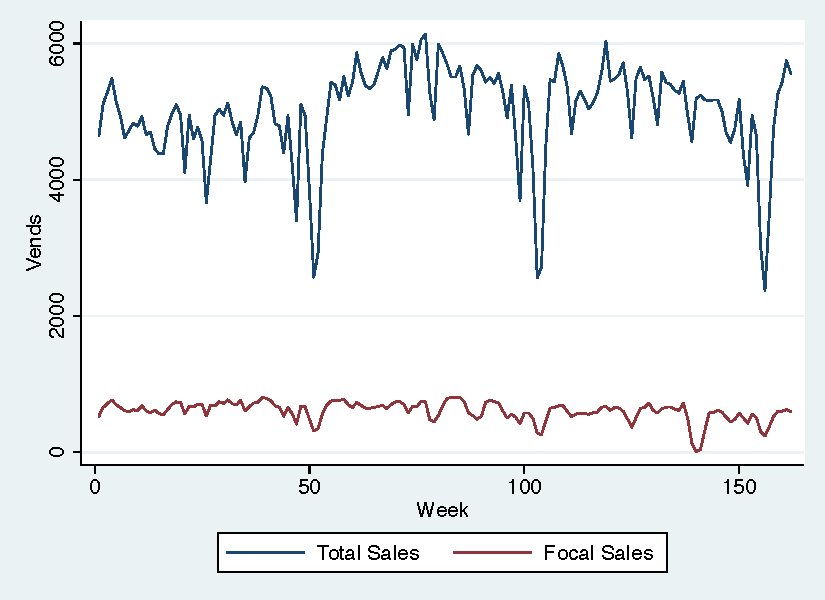
\includegraphics[width=4in]{./resources/figure1.pdf}
\end{center}
\end{frame}

\begin{frame}
\frametitle{A Matching Example}
Ideally we could just observe $M_t$ directly and use that as our matching variable $X$
\begin{itemize}
\item We didn't observe it directly and tried a few different measures:
\begin{itemize}
\item Sales at the soda machine next to the snack machine
\item Sales of salty snacks at the same machine (not substitutes for candy bars).
\item We used k-NN with $k=4$ to select control weeks -- notice we re-weight so that overall sales are approximately same (minus the removed product).
\end{itemize}
\item We also tried a more structured approach:
\begin{itemize}
\item Define controls weeks as valid IFF
\item Overall sales were weakly lower
\item Overall sales were not less than Overall Sales less expected sales less Snickers Sales.
\end{itemize}
\end{itemize}
\end{frame}


\begin{frame}
\begin{table}
\begin{center}
\tiny
\label{tab:nonparam}
\begin{tabular}{|l|rrrcrrcr|}
\hline
 & Control  & Control & Treatment& \hspace{-0.3in}& Treatment & Mean & \hspace{-0.3in} & \\
Product & Mean &  \%ile & Mean& \hspace{-0.3in} & \%ile &  Difference & \hspace{-0.3in}& \% $\Delta$\\
\hline \hline
\multicolumn{9}{|l|}{\emph{Vends}} \\ \hline
Peanut M\&Ms&359.9&73.6&478.3&\hspace{-0.3in}*&99.4&118.4& \hspace{-0.3in}*&32.9\\
Twix Caramel&187.6&55.3&297.1&\hspace{-0.3in}*&100.0&109.5& \hspace{-0.3in}*&58.4\\
Assorted Chocolate&334.8&66.7&398.0&\hspace{-0.3in}*&95.0&63.2& \hspace{-0.3in}*&18.9\\
Assorted Energy&571.9&63.5&616.2& \hspace{-0.3in}&76.7&44.3 & \hspace{-0.3in} &7.8\\
Zoo Animal Cracker&209.1&78.6&243.7&\hspace{-0.3in}*&98.1&34.6& \hspace{-0.3in}*&16.5\\
Salted Peanuts&187.9&70.4&216.3&\hspace{-0.3in}*&93.7&28.4 & \hspace{-0.3in} &15.1\\
Choc Chip Famous Amos&171.6&71.7&193.1&\hspace{-0.3in}*&95.0&21.5& \hspace{-0.3in}*&12.5\\
Ruger Vanilla Wafer&107.3&59.7&127.9& \hspace{-0.3in}&78.6&20.6& \hspace{-0.3in}*&19.1\\
Assorted Candy&215.8&43.4&229.6& \hspace{-0.3in}&60.4&13.7& \hspace{-0.3in}&6.4\\
Assorted Potato Chips&279.6&64.2&292.4&\hspace{-0.3in}*&66.7&12.8& \hspace{-0.3in}&4.6\\
Assorted Pretzels&548.3&87.4&557.7&\hspace{-0.3in}*&88.7&9.4& \hspace{-0.3in}&1.7\\
Raisinets&133.3&66.0&139.4& \hspace{-0.3in}&74.2&6.1& \hspace{-0.3in}&4.6\\
Cheetos&262.2&60.1&260.5& \hspace{-0.3in}&58.2&-1.8& \hspace{-0.3in}&-0.7\\
Grandmas Choc Chip&77.9&51.3&72.5& \hspace{-0.3in}&37.8&-5.4& \hspace{-0.3in}&-7.0\\
Doritos&215.4&54.1&203.1& \hspace{-0.3in}&39.6&-12.3& \hspace{-0.3in}*&-5.7\\
Assorted Cookie&180.3&61.0&162.4& \hspace{-0.3in}&48.4&-17.9& \hspace{-0.3in}&-10.0\\
Skittles&100.1&62.9&75.1&\hspace{-0.3in}*&30.2&-25.1& \hspace{-0.3in}*&-25.0\\
Assorted Salty Snack&1382.8&56.0&1276.2&\hspace{-0.3in}*&23.3&-106.7& \hspace{-0.3in}*&-7.7\\
Snickers&323.4&50.3&2.0&\hspace{-0.3in}*&1.3&-321.4& \hspace{-0.3in}*&-99.4\\ \hline
Total&5849.6&74.2&5841.3& \hspace{-0.3in}&73.0&-8.3& \hspace{-0.3in}&-0.1\\
\hline\end{tabular}
\end{center}
\tiny
Notes: Control weeks are selected through the-neighbor matching using four control observations for each treatment week.  Percentiles are relative to the full distribution of control weeks.
\end{table}
\end{frame}



\begin{frame}
\frametitle{Exercises}
\begin{itemize}
\item This would be a good time to work through the vignette for \texttt{cobalt}
 \url{https://cran.r-project.org/web/packages/cobalt/vignettes/cobalt.html}
 \item Compare the ATE for the Lalonde data with the IPW, Nearest Neighbor, and Propensity Score estimates.
 \item Then start the homework
\end{itemize}
\end{frame}


\section{Difference in Differences}



\begin{frame}{Motivation: Recap Matching}
Matching estimators had some advantages:
\begin{itemize}
\item Limited assumptions on \alert{functional forms}
\item We could do nearest neighbor matching and use kernels to compute treatment effects
\end{itemize}
Matching estimators had some drawbacks:
\begin{itemize}
\item Treated patients were ``matched'' to control patients based only on \alert{observable characteristics}
\begin{itemize}
\item Ignored \alert{selection on unobservables}.
\end{itemize}
\item Relied on \alert{cross sectional} variation to construct a control group.
\end{itemize}
\end{frame}


\begin{frame}{Motivation}
IV estimators resolve some of those issues but
\begin{itemize}
\item Good IV are in short supply!
\end{itemize}
 Often (in this course at least) we have access to \alert{panel data}.
\begin{itemize}
\item What if we could use panel data to control for \alert{unobserved heterogeneity} within a treated individual/group?
\end{itemize}
\alert{Difference in Difference} estimators are like the opposite of matching
\begin{itemize}
\item \alert{Strong} assumptions on \alert{functional form}
\item but... allow for \alert{unobservable heterogeneity} in outcomes.
\end{itemize}
\end{frame}


\section{Intro to Difference in Difference}


\begin{frame}{Differences}
\begin{itemize}
  \item Consider using OLS to estimate
  \begin{align*}
  Y_{i}=\beta_{0}+\beta_{1}\cdot D_{i}+ \varepsilon_{i}
  \end{align*}
  when $D_i \in \left\{ 0,1\right\}$ is assigned randomly.

  \medskip
  \item From the OLS formula and a little algebra, we can show that
  \begin{align*}
  \hat{b}_1 = \bar{Y}_{1} - \bar{Y}_{0}
  \end{align*}
  where $\bar{Y}_{1}$ is the sample mean of $Y_i$ conditional on
  $D_i = 1$, and similarly $\bar{Y}_{1}$ is the sample mean conditional on $D_i = 0$.

  \medskip
  \item Note: this loops us back to the treatment effects setup, where
  we were comparing conditional means.

\end{itemize}
\end{frame}



\begin{frame}{Differences-in-Differences I}
\begin{itemize}
  \item {\bf Differences-in-differences} is a {\bf quasi-experimental} design
  that attempts to deal with selection by focusing how treatment and control
  groups change between two periods

  \smallskip
  \item Consider the model  
  \begin{align*}
  Y_{it}=\beta_{0}+\beta_{1} \cdot D_{it}+\boldsymbol{\beta}_2' {\bf X}_{i}+ \beta_{post}  Post_t  + \varepsilon_{it},
  \end{align*}
  and furthermore suppose that
  \begin{itemize}
    \item Some variables in ${\bf X}$ may be unobserved
    \item $D_{it}$ is not random and may be correlated with ${\bf X}_{i}$
    \item $Post_t$ is a dummy variable for the post-treatment period $t=2$
    \item Each individual $i$ is observed (at least) twice
    \item For some individuals, $D_{it}$ changes over time ({\bf natural experiment})
    \item ${\bf X}_{i}$ does not change over time
  \end{itemize}

\end{itemize}
\end{frame}


\begin{frame}{Differences-in-Differences II}
\begin{align*}
  Y_{it}=\beta_{0}+\beta_{1}\cdot D_{it}+\boldsymbol{\beta}_2' {\bf X}_{i} + \beta_{post}  Post_t  + \varepsilon_{it},
\end{align*}

\begin{itemize}
  \item Let $\Delta Y_{i}$ represent the change in $Y_{it}$ between two time periods:
  \begin{align*}
  \Delta Y_{i} = Y_{i2} - Y_{i1},
  \end{align*}
  and define $\Delta D_i$ and $\Delta \varepsilon_i$ similarly.

  \medskip
  \item A differenced regression equation:
  \begin{align*}
  \Delta Y_{i}=\beta_{post} + \beta_{1} \Delta D_{i}+ \Delta \varepsilon_{i}
  \end{align*}

\end{itemize}
\end{frame}


\begin{frame}{Differences-in-Differences III}
\begin{align*}
  \Delta Y_{i}=\beta_{post} + \beta_{1}  \cdot \Delta D_{i}+ \Delta \varepsilon_{i}
\end{align*}

\begin{itemize}
  \item Applying OLS to the differenced regression equation will provide unbiased
  estimates as long as
  \begin{align*}
  \E\left[ \Delta \varepsilon_{i} \mid \Delta D_{i} \right] =0.
  \end{align*}
  Exogeneity assumptions of this form are known as the {\bf parallel trends
  assumption}.

\end{itemize}
\end{frame}

\begin{frame}{Differences-in-Differences IV}
\begin{align*}
  \Delta Y_{i}=\beta_{post} + \beta_{1} \cdot \Delta D_{i}+ \Delta \varepsilon_{i}
\end{align*}
\begin{itemize}
  \item From before, recall that the OLS estimator for a simple experiment
  amounted to the difference in conditional means of the outcome variable.

  \medskip
  \item The same is true here, but now we start with an outcome variable that
  is differenced over time. Suppose that for some observations, $\Delta D_{i}=1$
  (treatment group), and for others $D_{i1}=D_{i2}=0$ (untreated group).
  \begin{align*}
\hat{b}_{1,DID}=\overline{\Delta Y}_{T}-\overline{\Delta Y}_{C}
\end{align*}
where $\overline{\Delta Y}_{T}$ is the conditional mean of $\Delta Y_{i}$
for the treatment group, and $\overline{\Delta Y}_{C}$ is the conditional
mean of $\Delta Y_{i}$ for the control group.

\end{itemize}
\end{frame}


\begin{frame}{The Appeal of DID}
\begin{itemize}
  \item The DID strategy is robust to a form of selection bias
  (when, the selection is related to persistent characteristics).
  Simple differences across treatment and control groups would not be.

  \medskip
  \item DID estimates are also robust to aggregate shocks or time effects. Simple differences
  over time for the treatment group would not be.

  \medskip
  \item DID can be used to study many ``natural experiments,'' where something
  changes for one group but not for an otherwise similar group.

\end{itemize}
\end{frame}

\section{A Famous Example: Card and Krueger (AER 1994)}

\begin{frame}{A Famous Example: Card and Krueger (AER 1994)}
\begin{itemize}
\item On April 1, 1992 NJ raises its minimum wage from $\$4.25\rightarrow \$5.05$ per hour.
\item Question: Econ 101 predicts this will \alert{reduce demand for low wage workers}
\begin{itemize}
\item Focus on fast food restaurants (since they pay min wage)
\item Focus on starting wage (avoid tenure, high turnover)
\end{itemize}
\item Survey 410 restaurants in NJ (treated group) and eastern PA (control group).
\item Idea: Compare \alert{change} in wages in $NJ$ to $PA$:  $\Delta_{DD} = \Delta_{NJ}- \Delta_{PA}$
\begin{itemize}
\item Wave 1: February 15-March 4, 1992
\item Wave 2: November 5 - December 31, 1992
\end{itemize}
\end{itemize}
\end{frame}

\begin{frame}{Balance Table: Covariates}
\begin{center}
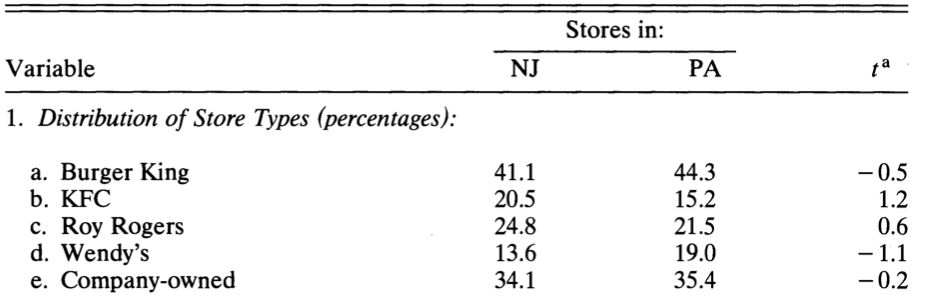
\includegraphics[width=2.25in]{./resources/ck_tab2b.png}\\
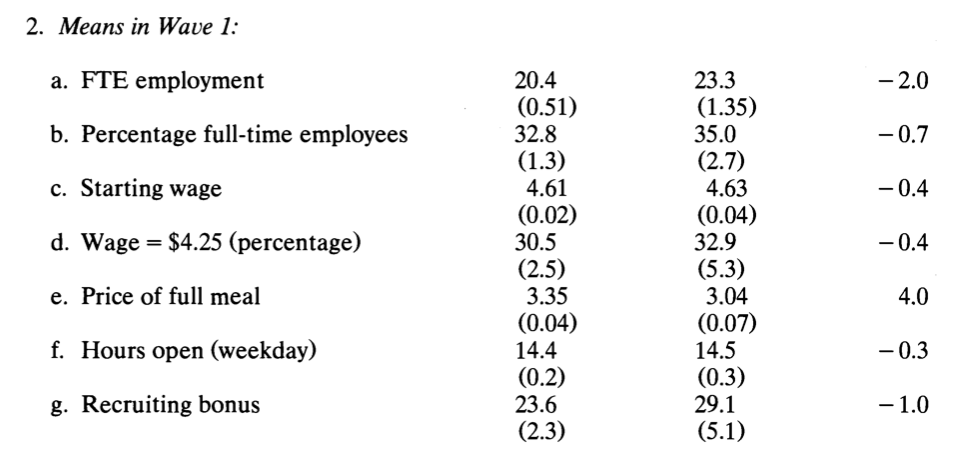
\includegraphics[width=2.25in]{./resources/ck_tab2c.png}\\
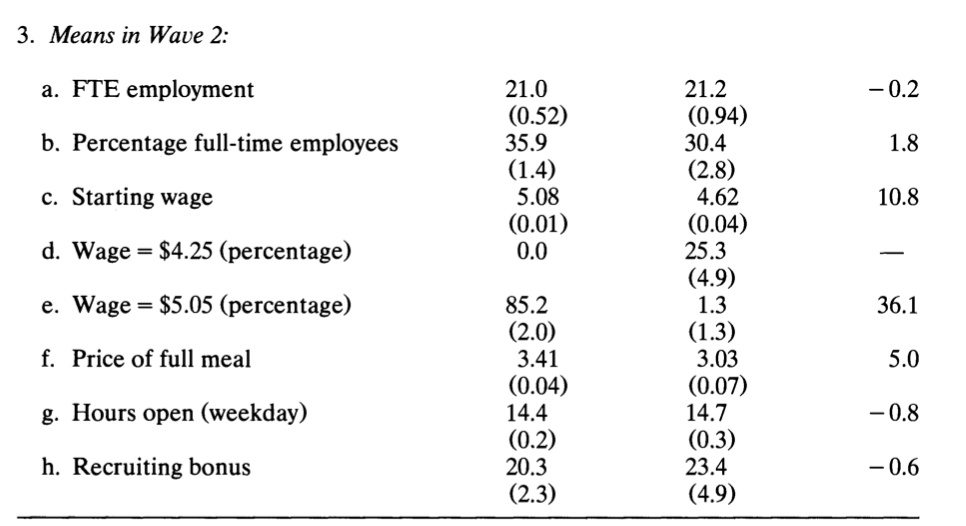
\includegraphics[width=2.25in]{./resources/ck_tab2a.png}
\end{center}
\end{frame}



\begin{frame}{Distribution of Wages}
\begin{center}
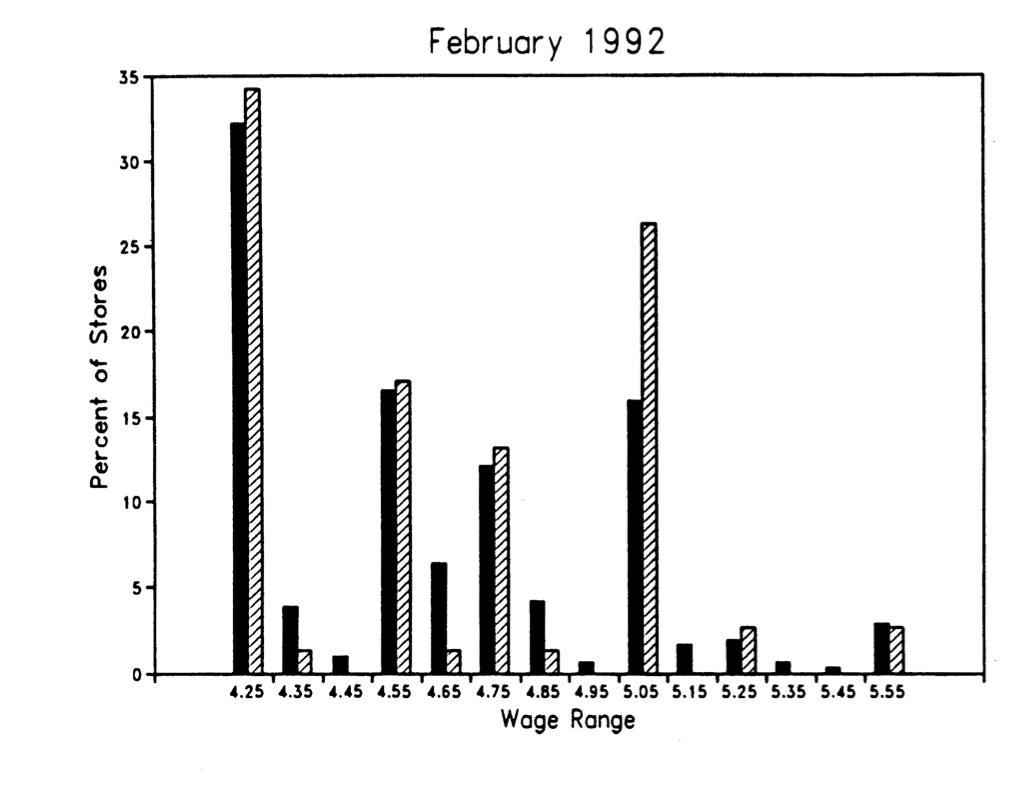
\includegraphics[width=2.75in]{./resources/ck_fig1b.png}
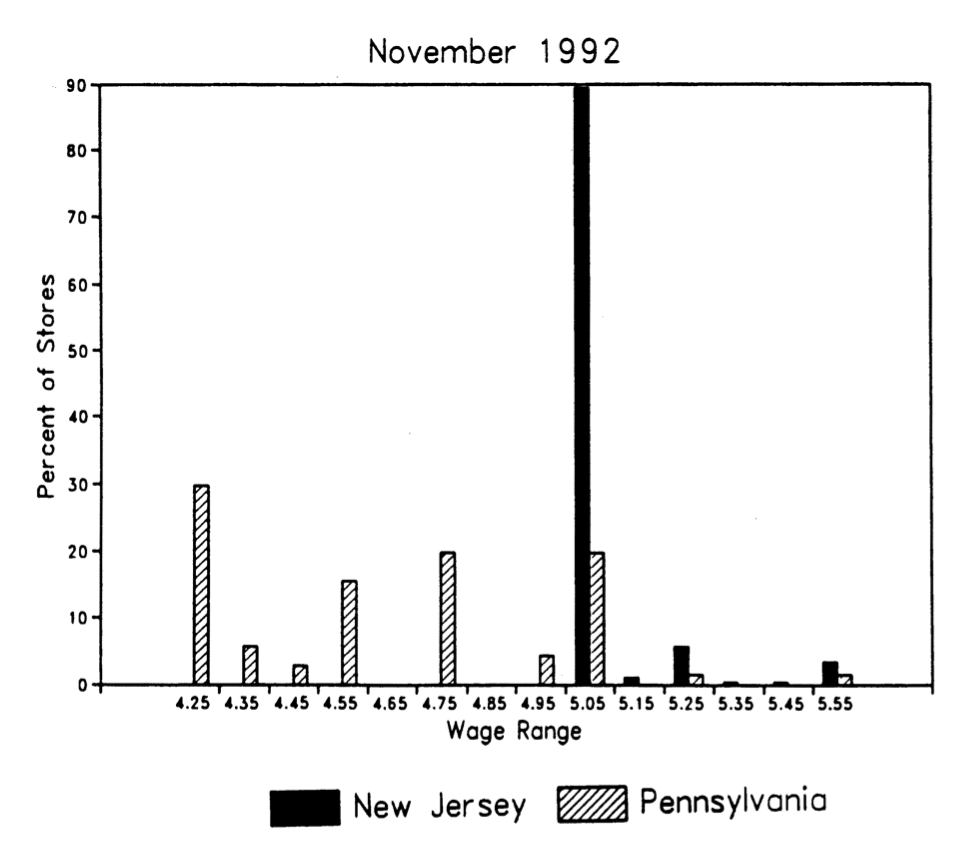
\includegraphics[width=2.5in]{./resources/ck_fig1a.png}
\end{center}
\end{frame}


\begin{frame}{Differences in Wages : 2 x 2 Table}
\begin{center}
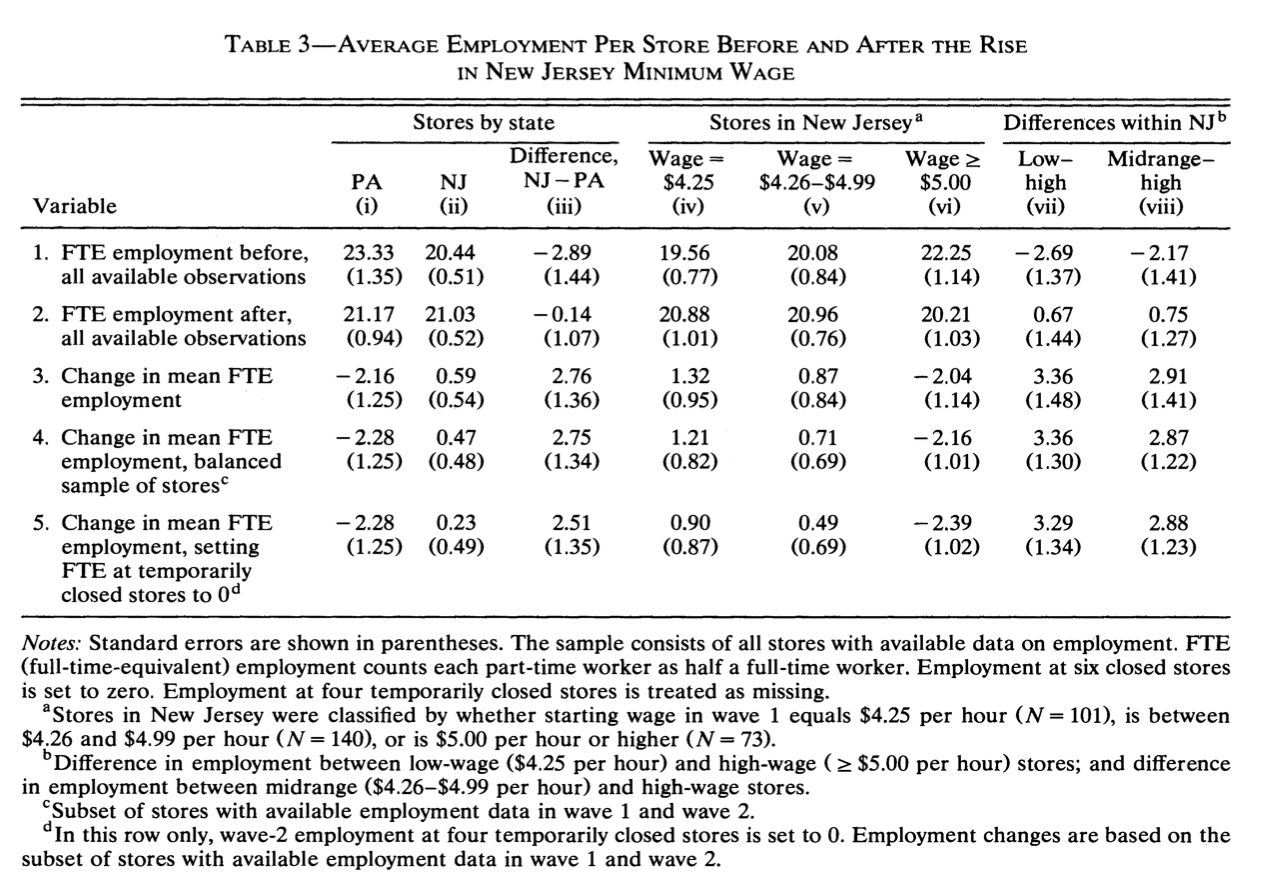
\includegraphics[width=4.25in]{./resources/ck_tab3.png}
\end{center}
\end{frame}

\begin{frame}{Outcome Equation}
\begin{itemize}
\item Differences lack any covariates (different fast food chains).
\item Also $\Delta_{PA}<0$ and $\Delta_{NJ} > 0$ (!)
\item Recall $i$ denotes stores, $t \in {1,2}$. Run the following regression:
\begin{align*}
Y_{it}&=\beta X_{it} +\alpha \cdot [i \in \text{NJ}] +  \gamma \cdot \text{After}_{t}  + \delta \cdot NJ_i \times After_{t} +u_{i}\\
Y_{it}&=\beta X_{it} +\alpha \cdot [\text{wage gap}_{i}] +  \gamma \cdot \text{After}_{t}  + \delta \cdot \text{wage gap}_{i} \times After_{t} +u_{i}
\end{align*}
\item $\alpha$ is mean difference between $NJ$ and $PA$
\item $\gamma$ is mean difference between period $1$ and $2$
\item $\delta$ is the parameter of interest, the \alert{difference in difference}
\item $\text{wage gap}_{i} = [\text{min wage}_{i,2}-w_{i1} ]_{+} =\max\{0, \text{min wage}_{i,2}-w_{i1}\} $.\\
 (How much do you need to raise $t=1$ wages to achieve minimum wage in $t=2$?)
\end{itemize}
\end{frame}

\begin{frame}{Differences in Wages}
\begin{center}
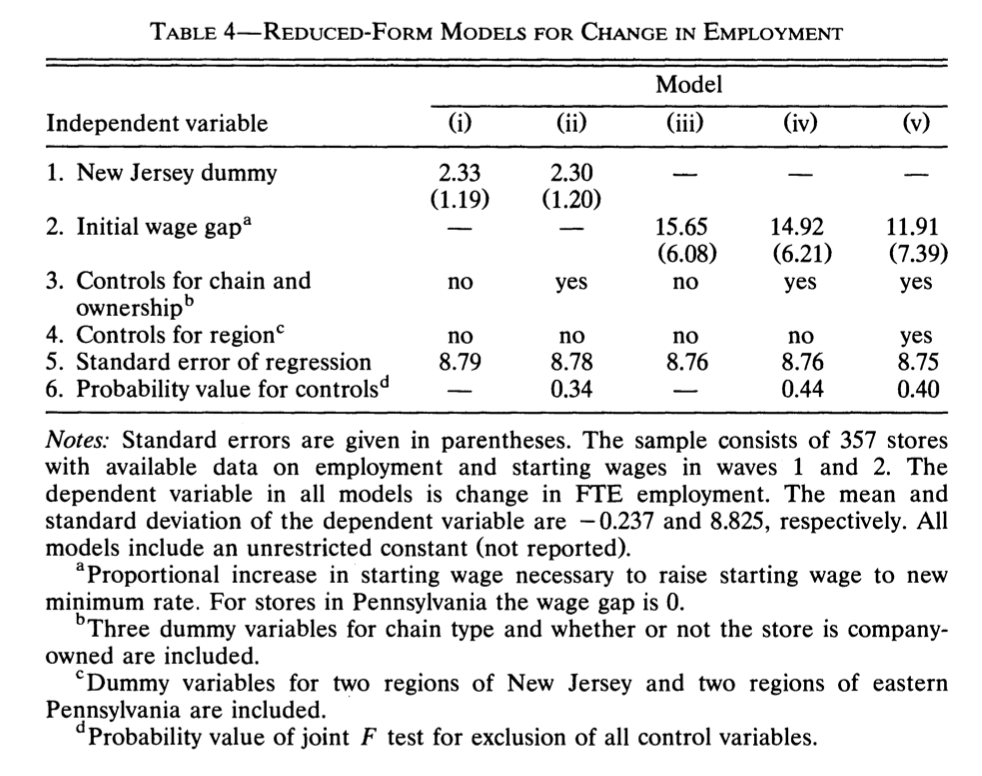
\includegraphics[width=4in]{./resources/ck_tab4.png}
\end{center}
\end{frame}


\begin{frame}{Parallel trends vs pre-trends}
\begin{itemize}
  \item When the data is available, researchers typically check {\bf pre-trends}
  as a way of motivating the parallel trends assumption.
  \begin{itemize}
    \item That is, look at how the control and treatment groups evolve in several
    periods preceding the time of treatment to see if they were changing in similar
    ways over time.
  \end{itemize}
  
  \smallskip
  \item This is a worthwhile check, and we should certainly worry about the plausibility
  of the parallel trends assumption if the pre-trends are not parallel.
  
  \smallskip
  \item However, the parallel trends assumption is about what \emph{would have happened}
  immediately at the time of treatment in the absence of treatment, not about what
  happened before treatment. Thus, establishing parallel pre-trends {\bf does not} establish
  the parallel trends assumption.
  \begin{itemize}
  \item  Just as we can't test exogeneity within the OLS framework, we can't test
  the parallel trends assumption within the DiD framework. 
  \end{itemize}
\end{itemize}
\end{frame}

\begin{frame}{Parallel trends vs pre-trends: example}
Consider the NJ minimum wage study. Here's a concern that would not be assuaged by seeing parallel pre-trends:
\begin{itemize}
  \item  If the minimum wage changed 
  because a new administration was elected in NJ and they implemented a portfolio
  of new policies, then the minimum wage change might have been just one of several
  ways in which NJ and PA were diverging at the time.  
  
  \smallskip
  \item Some of the other policy changes might have led to greater labor force participation and/or
  incentivized businesses to hire more.
  
  \smallskip 
  \item Because of these other changes, we would expect NJ's restaurant employment to move
  differently from PA's in 1992 even if the minimum wage change had not happened.

  \smallskip
  \item This could all be true even if NJ and PA were evolving similarly before 1992. The point is that
    the treatment was one thing that diverged in 1992, and if one thing was diverging at that point,
    perhaps other things were also diverging. 
\end{itemize}
\end{frame}




\begin{frame}{DID Experiments}
\begin{itemize}
  \item Recall that before we argued that experimental
  effects can be estimated with regressions using additional
  covariates (controls) even though they don't need to be.

  \medskip
  \item Similarly, they can be estimated using differences-in-differences
  rather than simple differences. They don't need to be, as with
  randomized treatment, the treatment and control groups should have
  similar baselines.

\end{itemize}
\end{frame}

\begin{frame}{NJ Minimum Wage Follow-Up}
\begin{itemize}
  \item The study has been controversial, and it has had a
  big impact on policy discussions.

  \medskip
  \item Card and Krueger update their conclusion
  in a 2000 follow up:
  \begin{quotation}
The increase in New Jersey's minimum wage probably
had no effect on total employment in New Jersey's
fast-food industry, and possibly had a small positive
effect.
  \end{quotation}

  \smallskip
  \item There have been \emph{many} criticisms of the paper,
  including studies showing that the result is not robust to the
  sample of stores and data source used, and concerns about
  the external validity of the focus on only fast food stores.

  \smallskip
  \item Also see studies based on Seattle's 2015 minimum wage change. 
\end{itemize}
\end{frame}



\section{A More General Method}



\begin{frame}{Difference in Difference: General Approach}
\begin{align*}
\text{Potential outcome in period } 1&=Y_{i 1}(0)\\
\text{Potential outcome in period } 2&=\left\{ \begin{array}{ll}
Y_{i 2}(1) & \text { if } D_{i 2}=1 \\ 
Y_{i 2}(0) & \text { if } D_{i 2}=0
\end{array}\right\}\\
\end{align*}
\begin{center}
\begin{tabular}{|c|c|c|}
\hline & Treatment & Control \\
\hline Before & $Y_{i 1}(0)$ & $Y_{i 1}(0)$ \\
After & $Y_{i 2}(1)$ & $Y_{i 2}(0)$ \\
\hline
\end{tabular}
\end{center}
We can write the outcome as:
\begin{align*}
Y_{i t}=D_{i t} \cdot Y_{i t}(1)+\left(1-D_{i t}\right) \cdot Y_{i t}(0)=D_{i t} \cdot\left(Y_{i t}(1)-Y_{i t}(0) \right)+Y_{i t}(0)
\end{align*}
\end{frame}

\begin{frame}{Difference in Difference: General Approach}
\small
Consider the first difference $\Delta Y_{it} = Y_{i2} - Y_{i1}$:
\begin{align*}
\Delta Y_{it}  = D_{i2} \cdot \left(Y_{i2}(1) - Y_{i2}(0) \right) +  Y_{i2}(0) - Y_{i1}(0)
\end{align*}
For treated group (first difference):
\begin{align*}
\E[\Delta Y_{it} \mid D_{i2}=1]  = \overbrace{\E\left[Y_{i2}(1) - Y_{i2}(0) \mid T_{i2}=1 \right]}^{\alert{ATT}} +  \overbrace{\E\left[Y_{i2}(0) - Y_{i1}(0) \mid D_{i2}=1 \right]}^{\alert{\gamma(1)}}
\end{align*}
For control group (second difference):
\begin{align*}
\E[\Delta Y_{it} \mid D_{i2}=0]  = \overbrace{\E\left[Y_{i2}(0) - Y_{i1}(0) \mid D_{i2}=0 \right]}^{\alert{\gamma(0)}}
\end{align*}
The DiD (difference in difference) estimator
\begin{align*}
\Delta_{DD} = \E[\Delta Y_{it} \mid D_{i2}=1]  - \E[\Delta Y_{it} \mid D_{i2}=0]  
\end{align*}
\end{frame}



\begin{frame}{Difference in Difference: Parallel Trends}
\small
\begin{itemize}
\item If $\gamma(1) = \gamma(0)$ then the DiD estimator cancels and we are left with the $\Delta_{DD} = \text{ATT}$.
\item This is the \alert{parallel trends assumption}
\begin{align*}
\E\left[Y_{i2}(0) - Y_{i1}(0) \mid D_{i2}=0 \right] = \E\left[Y_{i2}(0) - Y_{i1}(0) \mid D_{i2}=1 \right]
\end{align*}
\item Absent the treatment effect, both treatment and control would evolve identically over time.
\item But, treatment and control groups can start from very different places...
\begin{align*}
\E\left[Y_{i t}(0) \mid D_{i 2}=1\right] \neq E\left[Y_{i t}(0) \mid D_{i 2}=0\right], t=1,2
\end{align*}
\item And have selection on treatment effects...
\begin{align*}
\E\left[Y_{i 2}(1)-Y_{i 2}(0) \mid D_{i 2}=1\right] \neq \E\left[Y_{i 2}(1)-Y_{i 2}(0) \mid D_{i 2}=0\right]
\end{align*}
\end{itemize}
\end{frame}


\begin{frame}{Parallel Trends}
\begin{figure}
\centering
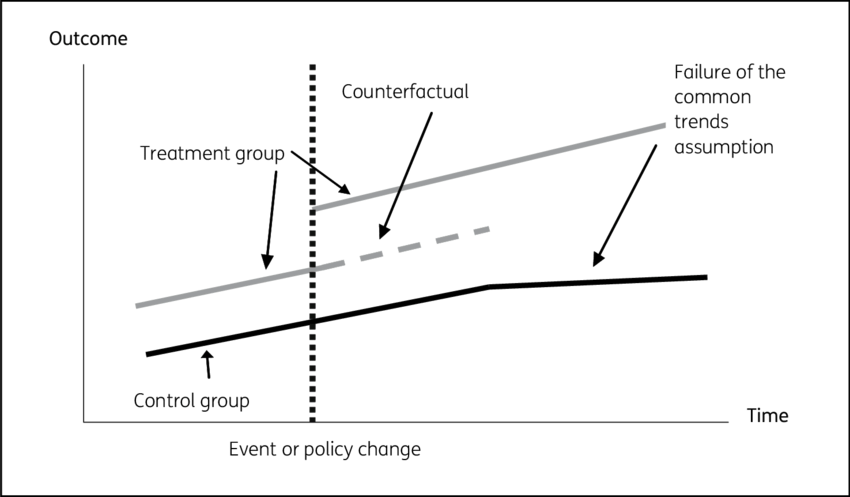
\includegraphics[width=5in]{./resources/common_trend.png}
\end{figure}
\end{frame}



\begin{frame}{Difference in Differences: Limitations}
\begin{enumerate}
\item Functional form restrictions
\begin{itemize}
\item \alert{Parallel trends} assumes that absent treatment that we add $\gamma_2 - \gamma_1$ to each unit
\item Because this is \alert{additive} it is not invariant to transformations $f(Y_{it})$ (ie: taking logs)
\end{itemize}
\item Parallel Trend Assumption is \alert{not testable}
\begin{itemize}
\item Best we can hope is that it looks similar in the pre-period
\end{itemize}
\item Compositional Effects: the treatment may affect who is in each group
\begin{itemize}
\item Restaurants could close in NJ and open nearby in PA to avoid minimum wage.
\item A good job training program may lead to migration, etc.
\item One approach: redefine the population so that it doesn't endogenously respond to treatment
\begin{itemize}
\item Recover something, but probably not ATT anymore...
\end{itemize}

\end{itemize}

\end{enumerate}

\end{frame}

\begin{frame}{Checking Pre-Trend: Card Krueger (2000)}
\begin{figure}
\centering
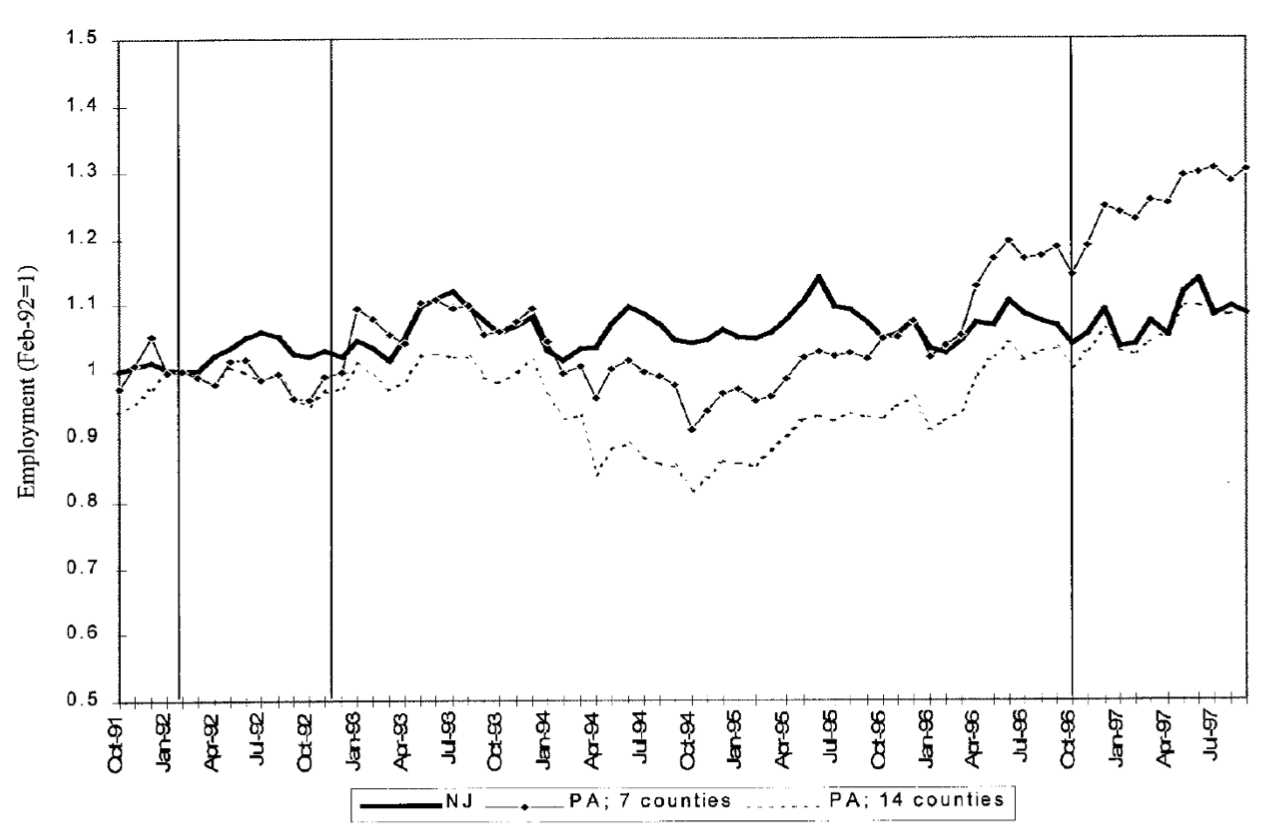
\includegraphics[width=4.5in]{./resources/card_krueger_2000.png}
\end{figure}
\end{frame}



\begin{frame}{Difference in Differences}
Just like in Card and Kruger, we can write as a regression equation:
\begin{align*}
 Y_{it} =\alpha_i +\gamma_t +\beta X_{it} + \delta_i D_{it}  + u_{it}
 \end{align*}
\begin{itemize}
\item Suppose we wish to evaluate a training program for those with low
earnings. Let the threshold for eligibility be $B$.
\item We have a panel of individuals and those with low earnings qualify for
training, forming the treatment group.
\item Those with higher earnings form the control group. 
\item Now the low earning group is low for two reasons
\begin{enumerate}
\item They have low permanent earnings ($\alpha_i$ is low) - this is accounted for by diff in diffs.
\item They have a negative transitory shock ($u_{i1}$ is low) - this is not accounted for by diff in diffs.
\end{enumerate} 
\end{itemize}
\end{frame} 

\begin{frame}{The ``Ashenfelter Dip'' (Heckman and Smith 2000)}
\begin{figure}
\centering
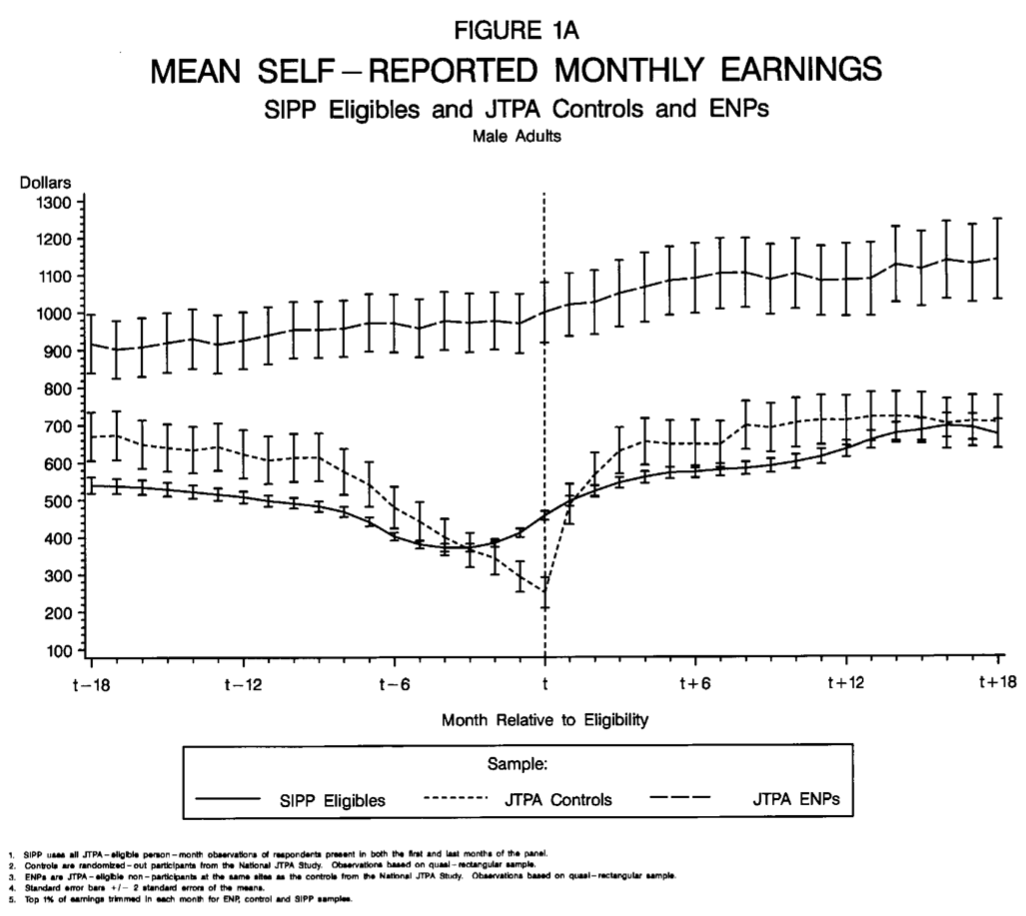
\includegraphics[width=4.25in]{./resources/ashenfelter_dip.png}
\end{figure}
\end{frame}

\begin{frame}{Difference in Differences}
\small
\begin{itemize}
\item  \#2 above violates the assumption {\small $\E[Y_{i2}(0) - Y_{i1}(0) | T] = \E[Y_{i2}(0) - Y_{i1}(0)]$}. 
\item To see why note that those participating into the program are such
that {\small $Y_{i0}(0) < B$}. Assume for simplicity that the shocks {\small $u$} are {\small $iid$}. Hence {\small $u_{i1} < B- \alpha_i - \gamma_1$}. 
This implies: 
{\small $$\E[Y_{i2}(0)- Y_{i1}(0) \mid D=1] = \gamma_2 = \gamma_1 - \E[u_{i1} \mid u_{i1} <  B-\alpha_i - \gamma_1]$$}
For the control group:
{\small $$\E[Y_{i2}(0) - Y_{i1}(0) \mid D=1] = \gamma_2 = \gamma_1 - \E[u_{i1} \mid u_{i1} >  B-\alpha_i - \gamma_1]$$}
So that:
\begin{align*}
& \E[Y_{i2}(0) - Y_{i1}(0) \mid D=1] - \E[Y_{i2}(0) - Y_{i1}(0) \mid T=0] =\\
&  \E[u_{i1} \mid u_{i1} >  B-\alpha_i - \gamma_1] - \E[u_{i1} \mid u_{i1} < B-\alpha_i - \gamma_1]  >0
  \end{align*}
 \item This is effectively regression to the mean: those unlucky enough to have a bad shock recover and show greater growth relative to those with a good shock. The nature of the bias depends on the stochastic properties of the shocks and how individuals select into training.
\end{itemize}
\end{frame} 

% \begin{frame}{Difference in Differences}
% Ashefelter (1978) was one of the first to consider difference in differences to evaluate training programs.
% 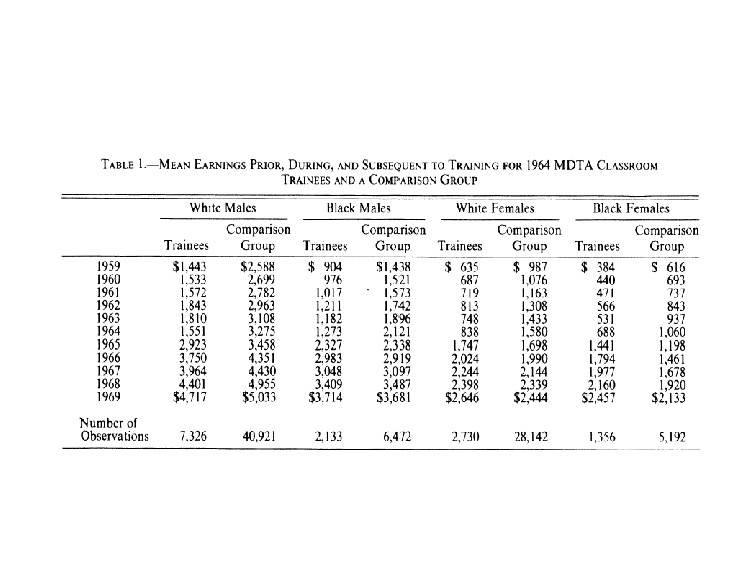
\includegraphics[scale=1]{./resources/ashefelter1.pdf}
% \end{frame}

% \begin{frame}{Difference in Differences}
% Ashenfelter (1978) reports the following results.
% \begin{figure}
% \centering
% 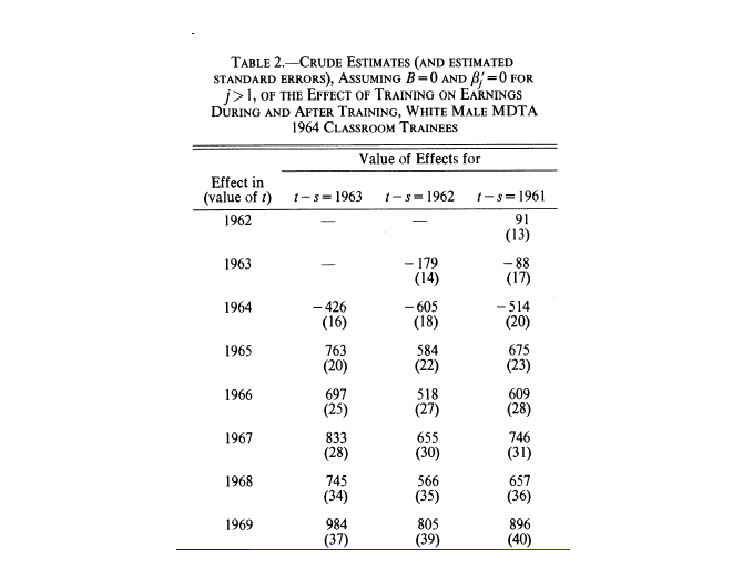
\includegraphics[scale=.85]{./resources/ashefelter2.pdf}
% \end{figure}
% \end{frame}

\begin{frame}{Difference in Differences}
\begin{itemize}
\item The assumption on growth of the non-treatment outcome being independent of assignment to treatment may be violated, but it may still be true conditional on $X$.
\item Consider the assumption
$$ \E[Y_{i2}(0)- Y_{i1}(0) \mid X,T] = \E[Y_{i2}(0)- Y_{i1}(0) \mid X] $$ 
\item This is just matching assumption on a redefined variable, namely the growth in the outcomes. In its simplest form the approach is implemented by running the regression
$$ Y_{it} = \alpha_i + \gamma_t + \delta_i D_{it} + \beta_t' X_i + u_{it}$$ 
which allows for differential trends in the non-treatment growth depending on $X_i$. More generally one can implement propensity score matching on the growth of outcome variable when panel data is available.
\end{itemize}
\end{frame}

\section{Variants}

\begin{frame}{Difference in Difference in Difference}
The triple difference is also a thing:
\begin{itemize}
\item Suppose that we have: before/after, treated-state/untreated-state, treated-group (men)/ untreated-group women.
\item We can compute two D-i-D here: $\Delta_{DDD} = \Delta_{DD,state} - \Delta_{DD,gender}$ 
\item Literally difference, the difference in differences estimators.
\item As a regression: interpret the triple-interaction term (make sure to control for ALL double interactions).
\end{itemize}
\end{frame}




\begin{frame}{DID with Time-Varying Covariates}
\begin{itemize}
  \item Suppose individuals have time-varying observable covariates:
  \begin{align*}
  Y_{it}=\beta_{0}+\beta_{1}\cdot D_{it}+\boldsymbol{\beta}_2' {\bf X}_{it} + \varepsilon_{it},
  \end{align*}

  \item We can still estimate $\beta_{1}$ with a differenced linear regression,
  \begin{align*}
  \Delta Y_{i}=\beta_{1} \cdot \Delta D_{i}+\boldsymbol{\beta}_2' \Delta {\bf X}_{it} + \Delta \varepsilon_{i}
  \end{align*}
  noting that the exogeneity assumption becomes
  \begin{align*}
\E\left[\Delta\varepsilon_{i}\left|\left(\begin{array}{c}
\Delta D_{i}\\
\Delta\mathbf{X}_{i}
\end{array}\right)\right.\right]=0
\end{align*}

  \item The estimate of $\beta_{1}$ here does not correspond to a simple
  difference in differences,
  but people still describe this sort of estimation strategy as DID.
  Given Frisch-Waugh, it's still DID after controlling for ${\bf X}$.


\end{itemize}
\end{frame}

\begin{frame}{Staggered DID}
\begin{itemize}
  \item A {\bf staggered diff-in-diff} involves different groups being
    treated at different points in time. Typically, these models are
    estimated with a linear regression with two-way fixed effects. (More
    on this when we get to panel data.) 

  \medskip
  \item See \href{https://www.sciencedirect.com/science/article/pii/S0304407620303948}{Callaway and Sant'Anna}, 
    \href{https://academic.oup.com/ectj/article/26/3/C1/6604378}{de Chaisemartin and D'Haultfoeuille (2023)}
    on why this is not a valid strategy in the presence of heterogeneous
    treatment effects and for alternative estimators. (More on this in Econometrics II)

\end{itemize}
\end{frame}

\section{Synthetic Control}



\begin{frame}{Motivation: Recap}
Difference in Difference approaches have some drawbacks:
\begin{itemize}
\item We need to really believe \alert{parallel trends}
\begin{itemize}
\item Is $\Delta PA$ really a good counterfactual for  $\Delta NJ$?
\item Obvious question: why not pick $\Delta DE$ or $\Delta NY$?
\item Measured effect shouldn't change if our assumption is valid (but it probably will!)
\end{itemize}
\item With multiple treated individuals we can use 2WFE estimator
\begin{align*}
y_{it} = \beta X_{it} + \delta_i \cdot T_{it} +  \gamma_i + \gamma_t + u_{it}
\end{align*}
\vspace{-0.8cm}
\begin{itemize}
\item It assumes \alert{additivity} of FE $\gamma_i + \gamma_t$ are independent!
\item States have different baseline levels $\gamma_i$ but evolution over time is common $\gamma_t$.
\item Turns out it doesn't really generalize the diff-in-diff with $I > 2$ (Imai and Kim 2020).
\end{itemize}            
\end{itemize}              
\end{frame}


\begin{frame}{Motivation: Recap}
Matching Estimators had drawbacks too:
\begin{itemize}
\item We need to believe in as if random-assignment conditional on $X$
\item CIA: $\{Y_i(1), Y_i(0)\} \perp T_i | X_i$.
\end{itemize}
But we could use pretty flexible methods in constructing our matched controls:           
\begin{itemize}
\item We could try to match on multiple dimensions of $X$.
\item $k\text{\textendash}NN$, kernels, etc.
\end{itemize}
What if we could use ideas from \alert{matching} to better satisfy something like our \alert{parallel trends} assumptions?
\end{frame}

\section{Example: Abadie, Diamond, Hainmueller (2010)}

\begin{frame}{The Question}
In 1988 California passes anti-smoking Prop 99
\begin{itemize}
\item increased excise tax by 25 cents per pack, 
\item earmarked the tax revenues to health and anti-smoking education budgets and funded anti-smoking ads
\item led to indoor smoking bans in restaurants and bars city by city
\end{itemize}
 What was the effect on per capita cigarette sales?
 \begin{itemize}
 \item Already a bunch of pre-existing trends.
 \item What is a good control for California?
 \end{itemize}
 Use state-level data from 1970-2000.
\end{frame}

\begin{frame}{The Idea}
Use a convex combination of other states to construct a \alert{synethetic counterfactual California}.\\
\begin{itemize}
\item We observe $Y_{it}, X_{it}, D_{it}$.
\item Assume only $i=1$ and $t > T_0$ are \alert{treated}.
\item Construct a \alert{donor pool} of potential controls subscripted by $j$.
\item Choose some \alert{weights} $w_j$ for each entity (state) in donor pool. How?
\begin{itemize}
\item Same $\mathbf{X_{1}} = \sum_j w_j \mathbf{X_{j}}$ as treated observations (like matching).
\item Same $\left({Y_{1,1},\ldots, Y_{1, T_0}} \right)= \sum_j w_j \cdot \left({Y_{j,1},\ldots, Y_{j,T_0}} \right)$ (like parallel trends).
\item Weights sum to one $\sum_j w_j = 1$ and maybe are non-negative (or not!)
\end{itemize}
\item Idea is to match all of the $X$'s and all of the $Y_{it}$'s in the \alert{pre-period}
\end{itemize}
\end{frame}

\begin{frame}{Covariate Balance}
\begin{center}
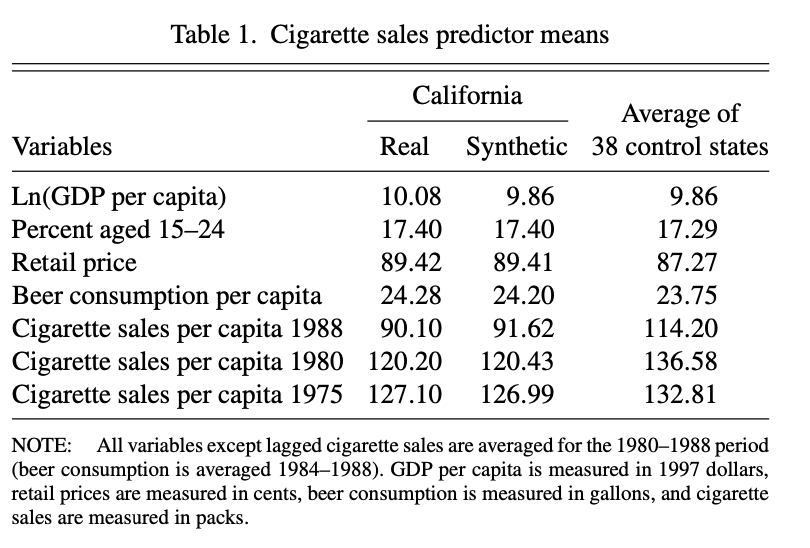
\includegraphics[width=4.5in]{./resources/abadie_1.png}
\end{center}
\end{frame}

\begin{frame}{Donor Weights}
\begin{center}
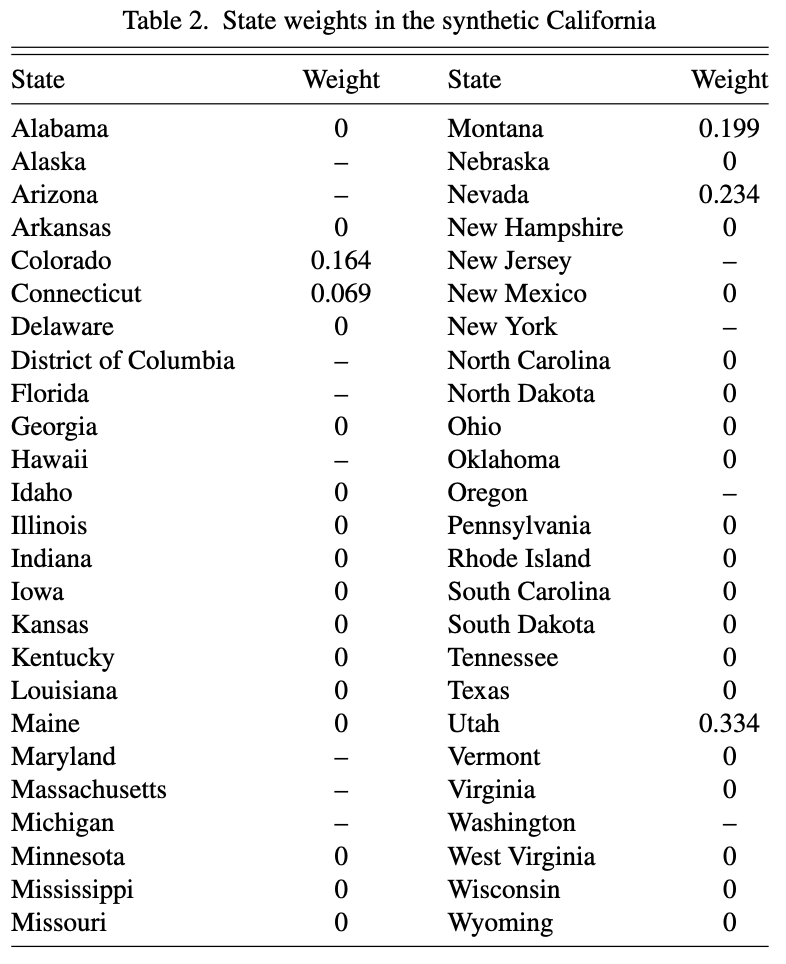
\includegraphics[width=2.5in]{./resources/abadie_2.png}
\end{center}
\end{frame}

\begin{frame}{Trend Check and Treatment Effects}
\begin{center}
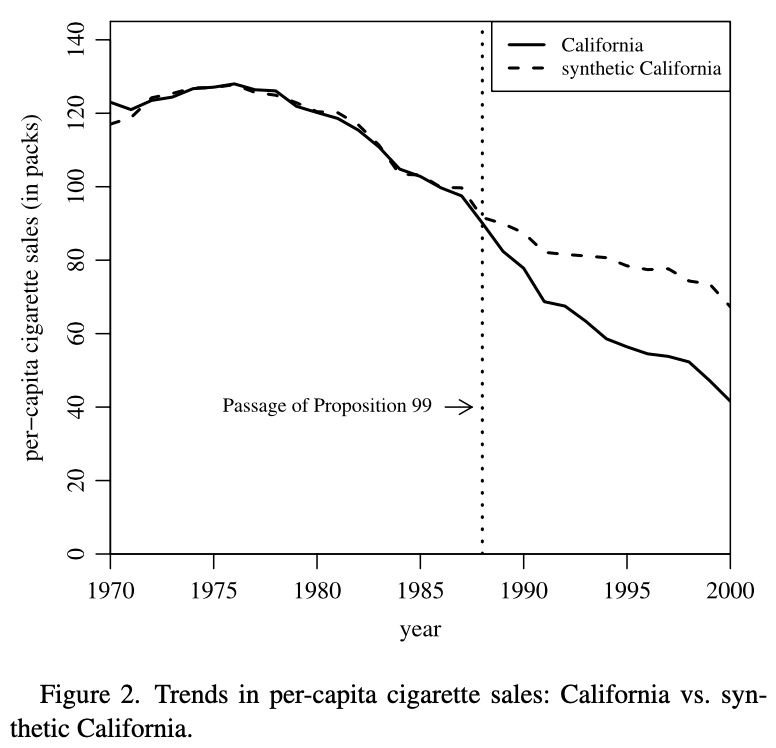
\includegraphics[width=2.75in]{./resources/abadie_3.png}
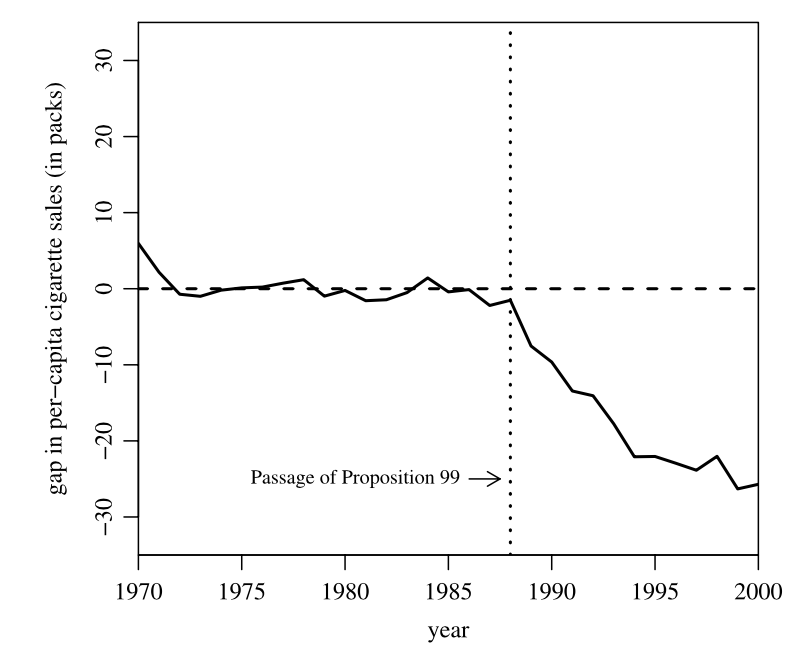
\includegraphics[width=2.75in]{./resources/abadie_4.png}
\end{center}
\end{frame}

\begin{frame}{But still some issues}
\begin{itemize}
\item How sensitive are weights estimates to different covariates?
\begin{itemize}
\item ``state-level measures of unemployment, income inequality, poverty, welfare transfers, crime rates, drug related arrest rates, cigarette taxes, population density, and numerous variables to capture the demographic, racial, and social structure of states''.
\end{itemize}
\item Can we run a \alert{placebo check}? Do we detect effects where we know there is a null effect?
\begin{itemize}
\item Put California in the donor pool.
\item Pick a state from the donor pool at pretend that receives the treatment after $T_0$
\item Choose $w_j$ following the synthetic control procedure.
\item Compute the treatment effects in the same way.
\item Repeat for all states in donor pool.
\item Compare \alert{mean-square prediction error} (MSPE) for $(Y_{1,1},\ldots,Y_{1,T_0})$
\item This doubles as \alert{inference}.
\end{itemize}
\end{itemize}
\end{frame}


\begin{frame}{Placebo Test}
\begin{center}
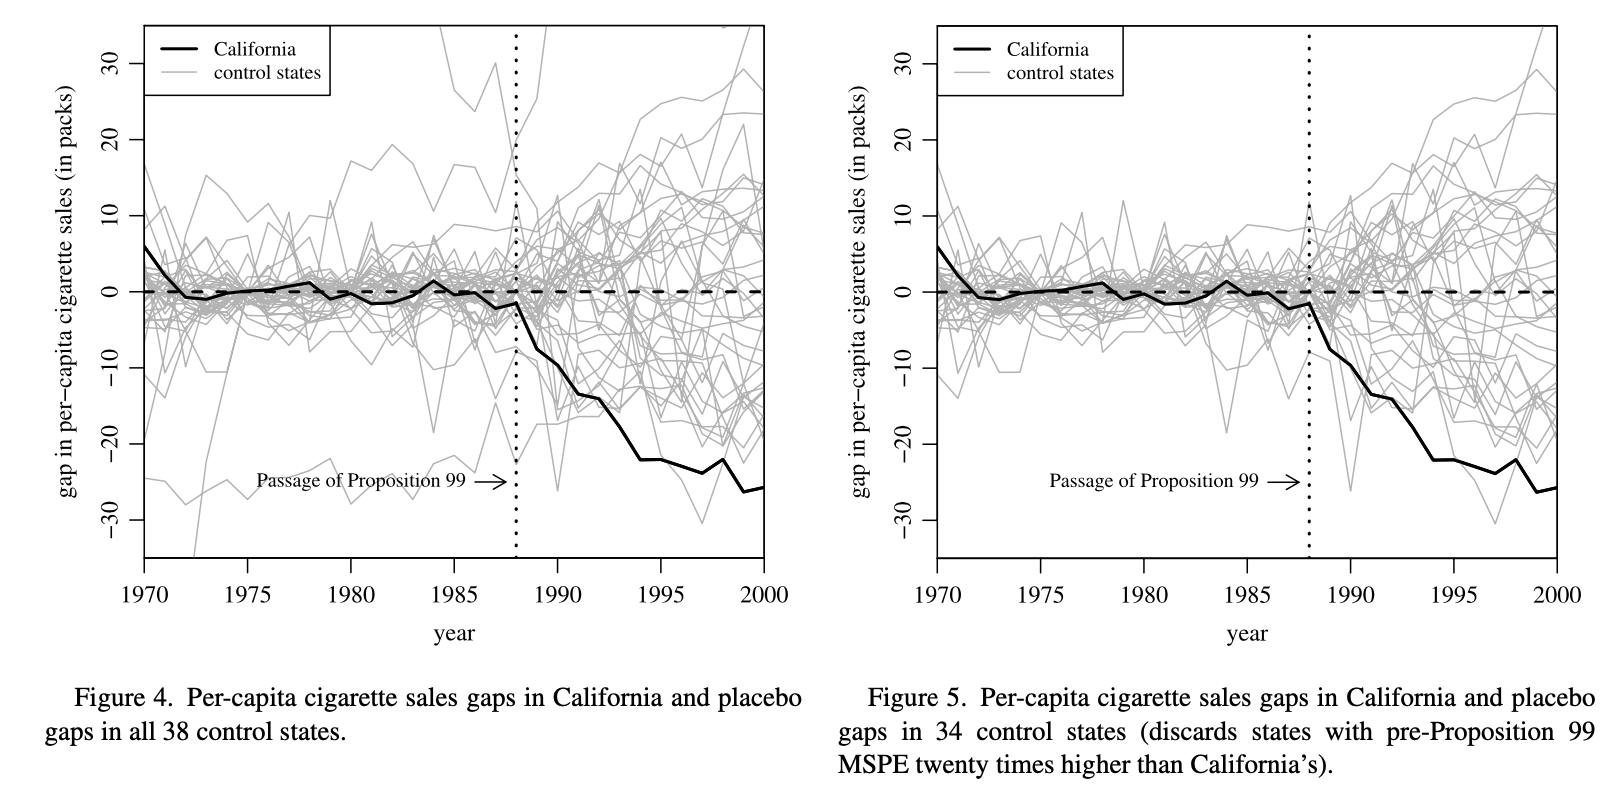
\includegraphics[width=5in]{./resources/abadie_5.png}
\end{center}
\end{frame}


\begin{frame}{More Placebo Tests: How unusual is the CA result?}
\begin{center}
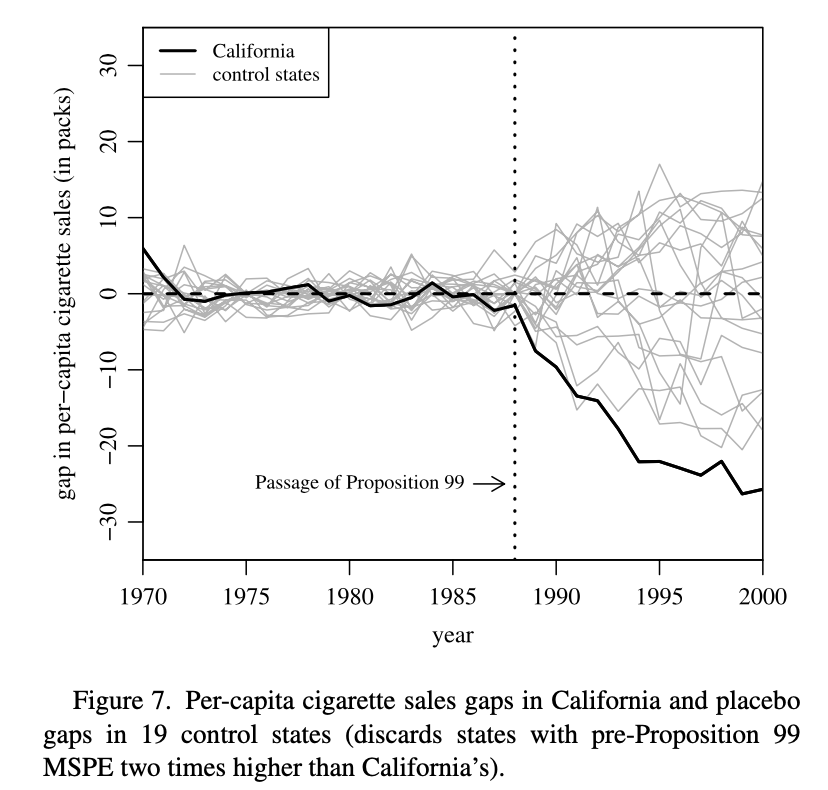
\includegraphics[width=2.75in]{./resources/abadie_6.png}
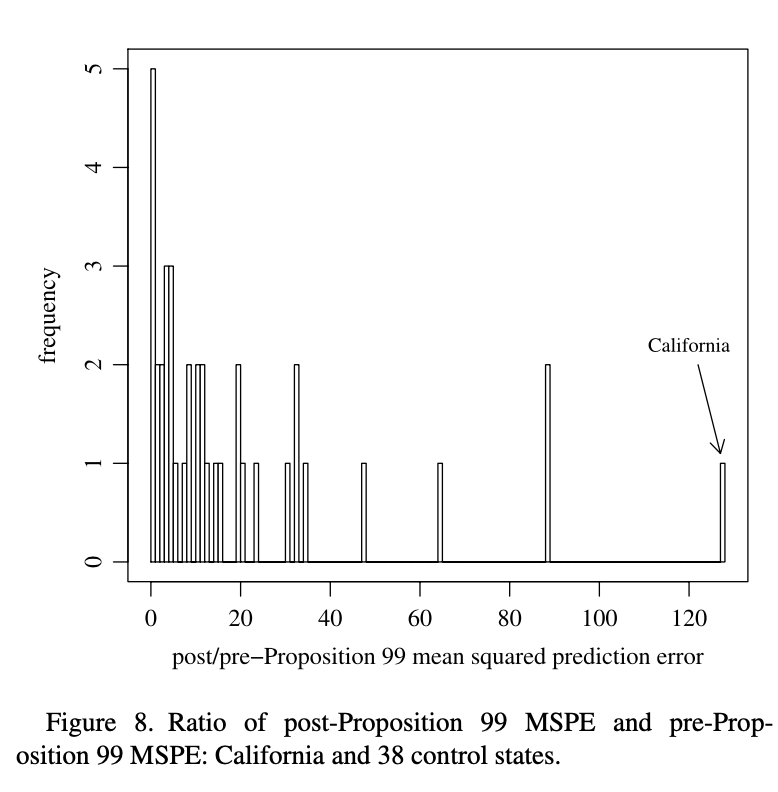
\includegraphics[width=2.75in]{./resources/abadie_7.png}
\end{center}
\end{frame}


\begin{frame}{More Formally}
We're going to break this down into three parts:
\begin{enumerate}
\item How do we estimate $w_j$?
\item Conditional on $\hat{w}_j$'s, how do we estimate the treatment effect?
\item What kinds of models are compatible?
\end{enumerate}
\end{frame}


\begin{frame}{A Starting Point}
Start with $D_{it} =1$ IFF $i =1$ and $t > T_0$:
\begin{align*}
Y_{it} = Y_{it}(0)  + \alpha_{it} \cdot D_{it}
\end{align*}
Estimate $\mathbf{\boldsymbol{\alpha}_1} =(\alpha_{1, T_0+1},\alpha_{1, T_0+2},\ldots,\alpha_{1,T}) $ (period by period treatment effect).\\
 For $t > T_0$:
\begin{align*}
\alpha_{1 t}=Y_{1 t}(1)-Y_{1 t}(0)=\underbrace{Y_{1 t}}_{\text{observed}}-\underbrace{Y_{1 t}(0)}_{\text{counterfactual}}
\end{align*}

\end{frame}

\begin{frame}{A Starting Point}
Consider the model
\begin{align*}
Y_{i t}(0)=\gamma_{t}+ \theta_{t} \mathbf{Z}_{i}+\lambda_{t} \mathbf{F}_{i}+u_{i t}
\end{align*}
\begin{itemize}
\item $\delta_t$ is the time fixed effect
\item $Z_i$ are the usual covariates (fixed in $i$ over time) with potentially time varying coefficients.
\item $F_i$ are $i$ specific \alert{unobserved factors}. Estimating these are complicated.
\item $\lambda_t$ are called \alert{factor loadings}.
\end{itemize}
This is a generalization of the usual additive $\gamma_t + \gamma_i$ fixed effects model called \alert{interactive fixed effects} (Bai 2009).
\end{frame}

\begin{frame}{Some Algebra}
So we define the synthetic observation as:
\begin{align*}
\sum_{j=2}^{J+1} w_{j} \underbrace{Y_{j t}(0)}_{\text{observed}}=\delta_{t}+\boldsymbol{\theta}_{t}\left(\sum_{j=2}^{J+1} w_{j} \mathbf{Z}_{j}\right)+\lambda_{t}\left(\sum_{j=2}^{J+1} w_{j} \boldsymbol{F}_{j}\right)+\sum_{j=2}^{J+1} w_{j} u_{j t}
\end{align*}
And the difference in untreated observations:
\begin{align*}
\begin{aligned}
Y_{1 t}(0)-\sum_{j=2}^{J+1} w_{j} Y_{j t}(0)\\
=\boldsymbol{\theta}_{t} \underbrace{\left( \mathbf{Z}_{1}-\sum_{j=2}^{J+1} w_{j} \mathbf{Z}_{j} \right)}_{\text{ match this directly}} 
&+\lambda_{t} \underbrace{\left(\boldsymbol{F}_{1}-\sum_{j=2}^{J+1} w_{j} \boldsymbol{F}_{j}\right)}_{\text{match indirectly:  }  (Y_{i,1},\ldots,Y_{i,T_0})}+\sum_{j=2}^{J+1} w_{j}\underbrace{\left(u_{1 t}-u_{j t}\right)}_{\text{Usual } \E[u_{it} \mid \mathbf{Z}_{it}, \mathbf{F}_{it} ]=0}
\end{aligned}
\end{align*}
\end{frame}


\begin{frame}{Some Algebra}
The goal is to match:
\begin{align*}
\mathbf{Z}_{1}= \sum_{j=2}^{J+1} w_{j} \mathbf{Z}_{j}, \quad
\mathbf{F}_{1} \approx \sum_{j=2}^{J+1} w_{j} \mathbf{F}_{j} 
\end{align*}
\begin{itemize}
\item The main result in the Abadie et. al (2010) paper proves that the above equation holds approximately if 
$$\left({Y_{1,1},\ldots, Y_{1,T_0}} \right)= \sum_j w_j \cdot \left({Y_{j,1},\ldots, Y_{j,T_0}} \right)$$
\item This frame generalizes the 2WFE model since we can use time dimension to difference them out.
\item We cannot difference out the $\lambda_t \mathbf{F}_i$.
\end{itemize}
\end{frame}


\begin{frame}{The Challenge}
Theory depends on matching:
\begin{align*}
\mathbf{Z}_{1}= \sum_{j=2}^{J+1} w_{j} \mathbf{Z}_{j}, \quad
\left({Y_{1,1},\ldots, Y_{1,T_0}} \right)= \sum_j w_j \cdot \left({Y_{j,1},\ldots, Y_{j,T_0}} \right)
\end{align*}
\begin{itemize}
\item One problem is the \alert{convex hull} problem. 
\begin{itemize}
\item There may be no $w_2,\ldots,w_J$ that satisfy the equations 
\end{itemize}
\item Instead choose $\mathbf{w}$ in a \alert{minimum distance sense} with some weighting matrix $\Omega$
\begin{itemize}
\item Can choose $\Omega$ to minimize variance of the resulting estimator.
\end{itemize}
\item Hard to fit crazy out of bounds values: can't match $CA$ population as linear combination of other states!
\end{itemize}
\end{frame}

\begin{frame}{Other Pitfalls}
Other things can go wrong
\begin{align*}
\mathbf{X}_{i}&=\left(\mathbf{Z}_{i}, Y_{i,1},\ldots, Y_{i,T_0} \right)\\
\arg \min_{w_2,\ldots, w_J}&  (\mathbf{X}_{i}-\sum_j w_j \mathbf{X}_{j})' \Omega  (\mathbf{X}_{i}-\sum_j w_j \mathbf{X}_{j}) \quad \text{ s.t. }  \sum_j w_j =1
\end{align*}

\begin{itemize}
\item Can get negative weights: what do those mean? 
\item We can rule them out $w_j \geq 0$ constraints but the problem becomes more difficult to solve.
\item This starts to look like a familiar LASSO problem: quadratic objective, $L_1$ penalty!
\item We shouldn't be surprised by sparse models.
\end{itemize}
\end{frame}

\begin{frame}{In practice}
\begin{itemize}
\item The R package \texttt{synth} or \texttt{tidysynth} and accompanying examples are a good start.
\item The R package \texttt{MSCMT} fixes some of the optimization issues in \texttt{synth}.
\begin{itemize}
\item When there is no set of feasible weights and the non-negativity constraint binds -- the problem is tricky to solve
\item \texttt{synth} can produce sub-optimal solutions (and slowly).
\end{itemize}

\end{itemize}

\end{frame}


\begin{frame}{A more unified view}
We can ask -- what are the implied regression weights for linear regression? What is $\E[Y_{1,t}(0) \mid \mathbf{X}]$?
\begin{itemize}
\item Get coefficients using just donor pool: $\widehat{\boldsymbol{B}}=\left(\overline{\boldsymbol{X}}_{0} \overline{\boldsymbol{X}}_{0}^{\prime}\right)^{-1} \overline{\boldsymbol{X}}_{0} \boldsymbol{Y}_{0}^{\prime}$
\item Predict $Y_{1,t}(0) = \widehat{\boldsymbol{B}}^{\prime} \overline{\boldsymbol{X}}_{1}$.
\item Same as synthetic control but with weights: $\boldsymbol{W}^{r e g}=\overline{\boldsymbol{X}}_{0}^{\prime}\left(\overline{\boldsymbol{X}}_{0} \overline{\boldsymbol{X}}_{0}^{\prime}\right)^{-1} \overline{\boldsymbol{X}}_{1}$ (Projection matrix).
\end{itemize}
Why? Remember, \alert{everything is a kernel} our prediction of $\E[Y \mid X]$ is always some weighted average of other $Y_j$'s.
\end{frame}

\begin{frame}{Additonal Applications}
\begin{itemize}
\item What is word of mouth effect of Superbowl ads? (Lovett, Peres, Xu QME 2019)
\begin{itemize}
\item Construct synthetic versions of brands that don't buy Superbowl ads
\end{itemize}
\item What is effect of soda tax on consumption in Berkeley, CA ? (Bollinger Sexton WP 2019).
\begin{itemize}
\item Construct synthetic drugstores, supermarkets, and convenience stores using two donor polls: inside CA and outside CA.
\end{itemize}
\item What are economic effects of German reunification?
\begin{itemize}
\item Now we need a counterfactual ``West Germany'' (!) \\
(Abadie, Diamond, and Hainmueller 2015)
\end{itemize}
\end{itemize}
\end{frame}

\begin{frame}{Weighting}
\begin{center}
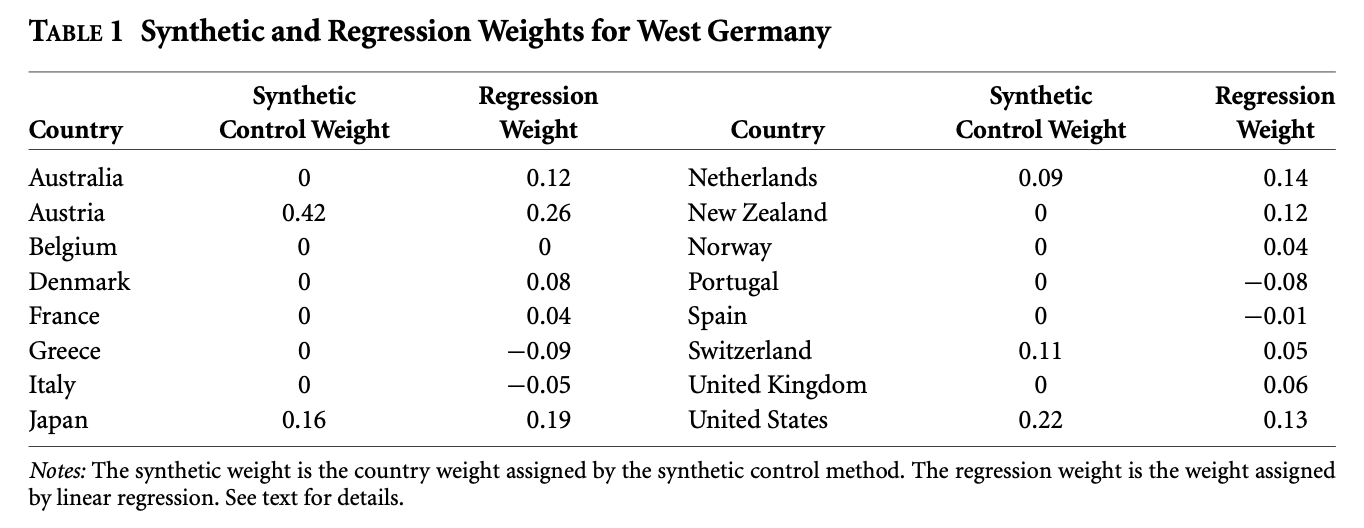
\includegraphics[width=6in]{./resources/germany_1.png}
\end{center}
\end{frame}

\begin{frame}{Balance Table}
\begin{center}
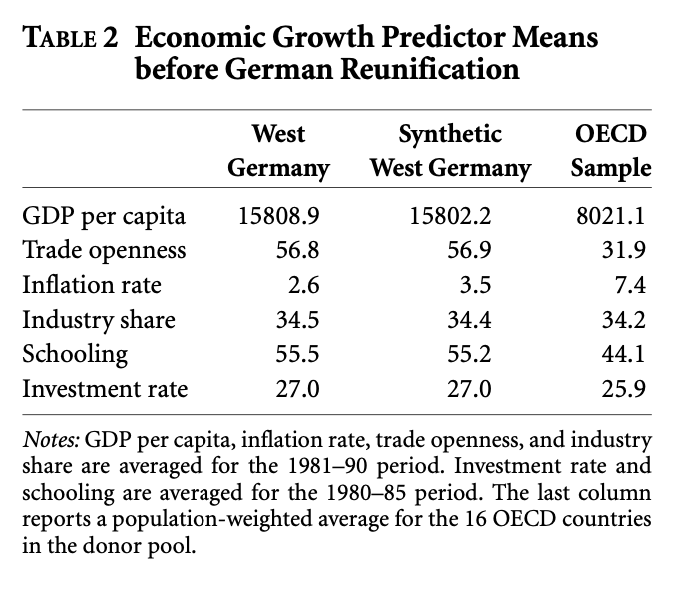
\includegraphics[width=3.2in]{./resources/germany_2.png}
\end{center}
\end{frame}

\begin{frame}{Treatment Effects}
\begin{center}
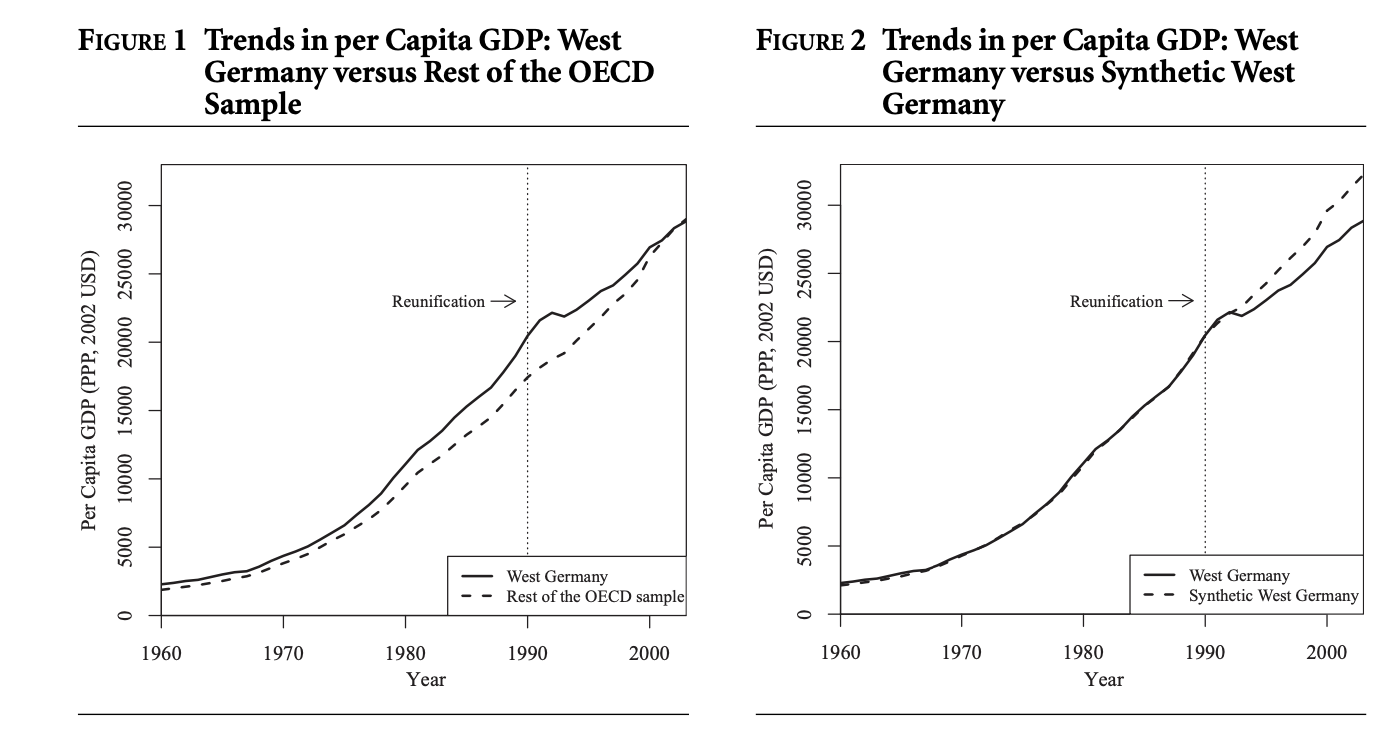
\includegraphics[width=5.5in]{./resources/germany_3.png}
\end{center}
\end{frame}


\begin{frame}{Treatment Effects and Placebo Timing}
\begin{center}
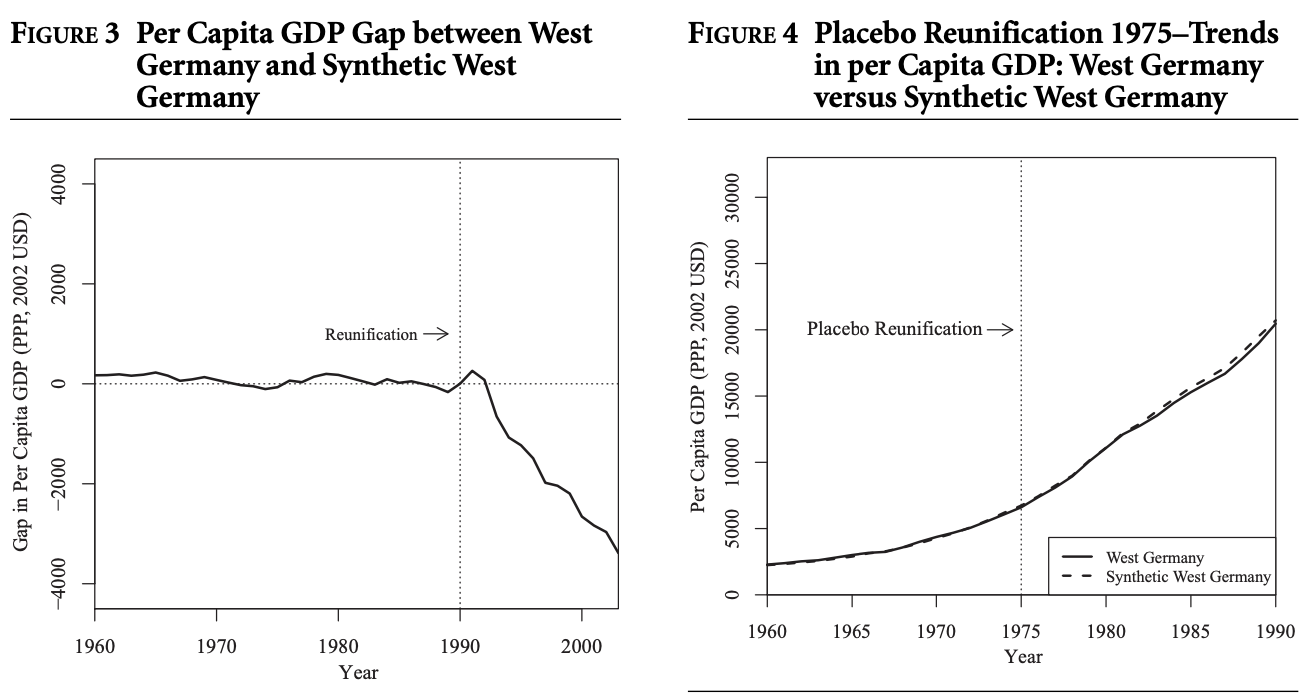
\includegraphics[width=5.5in]{./resources/germany_4.png}
\end{center}
\end{frame}

\begin{frame}{Treatment Effects and Placebo Timing}
\begin{center}
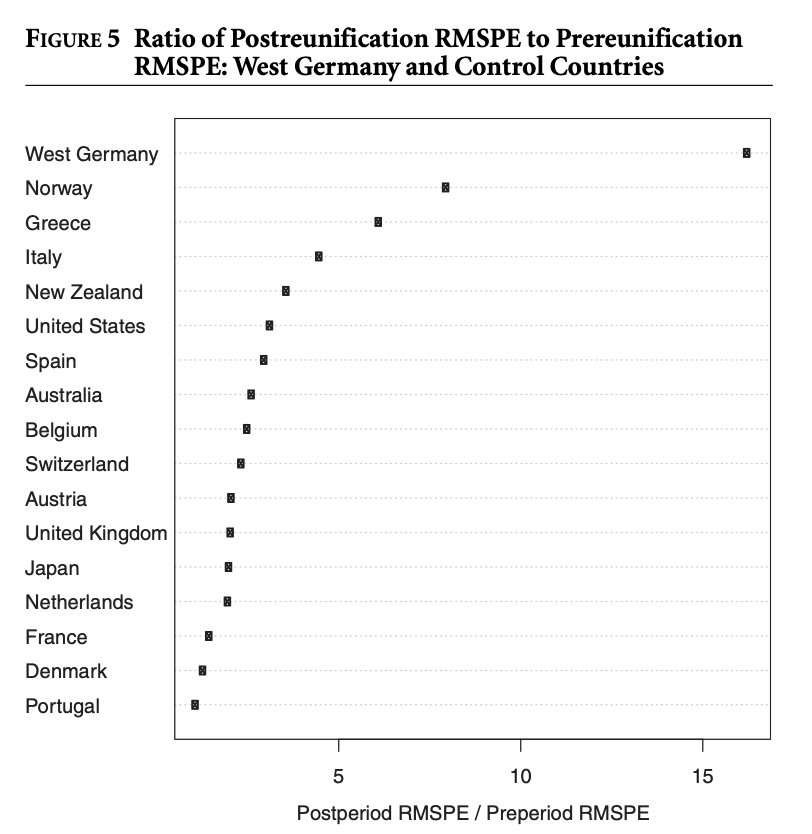
\includegraphics[width=2.8in]{./resources/germany_5.png}
\end{center}
\end{frame}

\section{Thanks}



\end{document}